% ============================================================================
%  CAPÍTULO 4 — RESULTADOS Y ANÁLISIS
% ============================================================================
\chapter{Resultados y análisis}
\label{cap:resultados}

En este capítulo se presentan los resultados obtenidos tras aplicar el
procedimiento de clustering a los egresos hospitalarios de establecimientos
públicos chilenos de alta y mediana complejidad durante el período 2019--2024.
Se reportan la selección de las particiones global del Nivel~1 y del núcleo
generalista del Nivel~2, junto con los perfiles clínico-operativos de los grupos
identificados.

Asimismo, se presentan la caracterización estadística posterior al
agrupamiento, el contraste con la clasificación administrativa del MINSAL, la
detección de hospitales atípicos y los análisis de sensibilidad algorítmica, de
elegibilidad, temporal y composicional.

\section{Universo de análisis y variables}
\label{sec:universo}

El universo final de análisis, tras aplicar los criterios de inclusión y
exclusión descritos en la Sección~\ref{sec:elegibilidad}, quedó constituido por
$n=65$ establecimientos. La caracterización de estos hospitales se realizó a
partir de una matriz integrada de 35 variables empleadas en el clustering. Esta
matriz combina 27 variables clínico-operativas directas, descritas en la
Tabla~\ref{tab:variables}, y ocho componentes principales de casuística
(\texttt{dim\_01} a \texttt{dim\_08}), que concentran el $72{,}3\%$ de la
varianza acumulada de la representación de casuística.

El indicador \texttt{peso\_medio\_cma} se reporta en la estadística descriptiva,
pero no se incorpora en la matriz de clustering. Su exclusión responde a que no
es una medida comparable cuando un establecimiento no registra actividad CMA,
pues en ese caso no corresponde interpretar la ausencia de casos como un peso
medio de complejidad nulo.

La Tabla~\ref{tab:resumen-matriz} sintetiza la composición de la matriz
institucional utilizada como entrada al procedimiento de clustering.

\begin{table}[htbp]
\centering
\caption{Composición de la matriz institucional de análisis.}
\label{tab:resumen-matriz}
\begin{tabular}{l r}
\toprule
\textbf{Dimensión} & \textbf{Valor} \\
\midrule
Hospitales (filas) & 65 \\
Período cubierto & 2019--2024 (6 años) \\
Registros de egreso procesados & 5{,}808{,}515 \\
\addlinespace
\multicolumn{2}{l}{\textit{Variables originales antes de la reducción PCA}} \\
\addlinespace
\quad Variables de gestión y producción & 6 \\
\quad Variables de diversidad diagnóstica & 2 \\
\quad Variables de CMA & 2 \\
\quad Variables de perfil funcional agregado & 18 \\
\quad Variables de casuística CIE-10 / CIE-9-MC / GRD & 63 \\
\quad \textbf{Total de variables originales} & \textbf{91} \\
\addlinespace
\multicolumn{2}{l}{\textit{Matriz final utilizada en el clustering}} \\
\addlinespace
\quad Variables clínico-operativas directas & 27 \\
\quad \textit{(6 gestión + 2 diversidad + 1 CMA + 18 perfil funcional)} & \\
\quad Componentes PCA de casuística & 8 \\
\quad \textbf{Total de variables en clustering} & \textbf{35} \\
\quad Varianza de casuística retenida con 8 componentes & 72{,}3\% \\
\bottomrule
\end{tabular}
\end{table}

\begin{table}[htbp]
\centering
\caption{Estadística descriptiva de las variables clínico-operativas de la red
hospitalaria ($n=65$).}
\label{tab:descriptiva-variables}
\begin{tabular}{l c c c c c}
\toprule
\textbf{Variable} & \textbf{Media} & \textbf{Desv. Est.} &
\textbf{Mínimo} & \textbf{Mediana} & \textbf{Máximo} \\
\midrule
Egresos por año & 12{,}518 & 7{,}644 & 2{,}663 & 10{,}667 & 39{,}066 \\
Estancia media (días) & 6{,}8 & 1{,}4 & 4{,}2 & 7{,}0 & 11{,}8 \\
Estancia mediana (días) & 3{,}4 & 0{,}778 & 2{,}0 & 3{,}0 & 7{,}0 \\
Peso medio GRD & 1{,}0 & 0{,}243 & 0{,}670 & 0{,}959 & 2{,}1 \\
Severidad media & 1{,}7 & 0{,}123 & 1{,}4 & 1{,}7 & 2{,}0 \\
Mortalidad media & 1{,}5 & 0{,}122 & 1{,}3 & 1{,}5 & 1{,}9 \\
Entropía GRD & 0{,}814 & 0{,}030 & 0{,}704 & 0{,}817 & 0{,}866 \\
Comorbilidades promedio & 4{,}7 & 0{,}983 & 2{,}8 & 4{,}5 & 7{,}1 \\
Tasa de CMA & 15{,}1\% & 7{,}9\% & 0{,}000\% & 14{,}3\% & 41{,}6\% \\
Peso medio CMA & 0{,}545 & 0{,}076 & 0{,}406 & 0{,}545 & 0{,}844 \\
CV de estancia & 2{,}0 & 0{,}435 & 1{,}2 & 1{,}9 & 3{,}0 \\
Edad mediana (años) & 42{,}4 & 10{,}9 & 4{,}0 & 42{,}0 & 64{,}2 \\
Pabellones promedio & 0{,}533 & 0{,}209 & 0{,}186 & 0{,}494 & 1{,}4 \\
\% Alta a domicilio & 87{,}5\% & 4{,}7\% & 75{,}9\% & 88{,}6\% & 98{,}0\% \\
\% Alta fallecido & 3{,}4\% & 1{,}2\% & 0{,}312\% & 3{,}4\% & 6{,}7\% \\
\% Alta traslado & 4{,}9\% & 2{,}9\% & 1{,}4\% & 3{,}8\% & 16{,}4\% \\
\% Estancia larga & 3{,}2\% & 1{,}4\% & 0{,}584\% & 3{,}4\% & 7{,}3\% \\
\% Femenino fértil & 30{,}6\% & 9{,}6\% & 1{,}8\% & 31{,}7\% & 47{,}6\% \\
\% Geriátrico & 25{,}9\% & 8{,}6\% & 0{,}000\% & 25{,}7\% & 48{,}3\% \\
\% Ingresos obstétricos & 18{,}2\% & 8{,}7\% & 0{,}000\% & 19{,}3\% & 34{,}7\% \\
\% Origen emergencia & 58{,}7\% & 18{,}0\% & 0{,}032\% & 61{,}8\% & 86{,}2\% \\
\% Origen referencia & 11{,}5\% & 10{,}7\% & 0{,}520\% & 9{,}2\% & 61{,}1\% \\
\% Pediátrico & 16{,}1\% & 18{,}2\% & 0{,}000\% & 14{,}1\% & 96{,}6\% \\
\% Programada & 21{,}3\% & 13{,}0\% & 1{,}0\% & 17{,}9\% & 81{,}6\% \\
\% Urgencia & 60{,}5\% & 11{,}4\% & 18{,}4\% & 60{,}9\% & 99{,}0\% \\
\% Uso de pabellón & 42{,}4\% & 9{,}3\% & 18{,}6\% & 42{,}8\% & 77{,}7\% \\
Proporción de egresos neonatales & 2{,}5\% & 1{,}4\% & 0{,}000\% & 2{,}7\% & 5{,}6\% \\
Tasa de prematurez & 6{,}5\% & 3{,}6\% & 0{,}000\% & 6{,}5\% & 13{,}1\% \\
\bottomrule
\end{tabular}
\end{table}

La Tabla~\ref{tab:descriptiva-variables} muestra una heterogeneidad importante
en el volumen de actividad, el perfil de pacientes y los indicadores clínicos de
los establecimientos analizados. Los egresos anuales varían entre 2{,}663 y 39{,}066
por hospital, lo que evidencia diferencias sustantivas en la escala asistencial.
Asimismo, la proporción de ingresos de urgencia presenta una media de
$60{,}5\%$ y alcanza un máximo de $99{,}0\%$, mientras que la proporción de
egresos pediátricos varía entre $0{,}0\%$ y $96{,}6\%$.

El peso medio GRD también presenta variación entre establecimientos, con valores
entre $0{,}670$ y $2{,}131$, al igual que los indicadores de edad, actividad
obstétrica, uso de pabellón, cirugía mayor ambulatoria y comorbilidades. Esta
heterogeneidad multidimensional motiva el uso de clustering como herramienta
exploratoria para identificar perfiles funcionales de hospitales con patrones de
actividad y casuística relativamente similares.

\section{Contribución de bloques a la geometría de distancia}
\label{sec:res-bloques}

La Tabla~\ref{tab:contribucion-bloques} descompone la suma de distancias
euclidianas cuadradas de la matriz preprocesada según los cuatro macro-bloques
definidos en la Sección~\ref{sec:bloques-variables}. El bloque
demográfico-obstétrico aporta $36{,}3\%$ de la distancia total, la fracción más
alta entre los bloques. Por tanto, la composición de demanda tiene una influencia
relevante en la geometría original y debe hacerse explícita al interpretar los
perfiles. No obstante, los otros tres bloques aportan conjuntamente el
$63{,}7\%$ de la distancia, por lo que la partición no puede atribuirse solo a
la demografía.

Dentro de ese bloque, la variable técnica \texttt{tasa\_partos} se reporta en
este documento como \emph{proporción de egresos neonatales}: corresponde a los
egresos hospitalarios con \texttt{CONDICIONDEALTANEONATO1} informada y no a un
conteo ni a una tasa clínica de partos atendidos. Su correlación con la
proporción de ingresos obstétricos es alta (Pearson $r=0{,}927$; Spearman
$\rho=0{,}926$; $n=65$), por lo que ambas variables contienen información
redundante respecto de la orientación obstétrico-neonatal. La correlación con la
proporción de egresos de mujeres fértiles también es alta, pero inferior al
umbral de redundancia predefinido ($\rho=0{,}876$). El análisis de sensibilidad
al retirar \texttt{tasa\_partos} modifica la solución ($ARI=0{,}635$;
$NMI=0{,}696$), por
lo que la redundancia no equivale a irrelevancia geométrica. Se conserva la
variable por compatibilidad con el diseño obstétrico-neonatal, pero el resultado
no se atribuye a una medida independiente de partos ni se interpreta como una
frontera robusta frente a especificaciones alternativas del bloque.

\begin{table}[htbp]
\centering
\caption{Contribución de los macro-bloques a la suma de distancias euclidianas
cuadradas en la matriz preprocesada.}
\label{tab:contribucion-bloques}
\begin{tabular}{l c c}
\toprule
\textbf{Bloque} & \textbf{Variables} & \textbf{Fracción de distancia} \\
\midrule
Gestión, diversidad y CMA & 9 & 15,1\% \\
Perfil operativo no demográfico & 11 & 27,7\% \\
Demográfico-obstétrico & 7 & 36,3\% \\
Componentes PCA de casuística & 8 & 20,9\% \\
\bottomrule
\end{tabular}
\end{table}

La Tabla~\ref{tab:sensibilidad-bloques} evalúa dos sensibilidades. La
ponderación por $1/\sqrt{p_b}$ por bloque conserva exactamente la partición
principal ($ARI=NMI=1{,}000$) y mejora marginalmente sus métricas internas.
En cambio, al excluir las siete variables demográfico-obstétricas, la
concordancia disminuye de forma importante ($ARI=0{,}571$; $NMI=0{,}599$): los
clústeres pediátrico y monográfico permanecen separados, pero seis hospitales
del núcleo y tres del grupo $C2$ cambian de agrupación. La menor cohesión de
esta solución (Silhouette $=0{,}238$ frente a $0{,}398$) indica que el bloque
excluido contribuye materialmente a la separación, por tanto, los perfiles no
deben interpretarse como independientes de la composición
demográfico-obstétrica.

\begin{table}[htbp]
\centering
\caption{Sensibilidad Ward $K=4$ a la ponderación por bloques y a la exclusión
del bloque demográfico-obstétrico. La concordancia se calcula respecto de la
partición base.}
\label{tab:sensibilidad-bloques}

\begin{tabular}{l c c c c c}
\toprule
\textbf{Escenario} & \textbf{Variables} & \textbf{Silhouette} &
\textbf{DB} & \textbf{ARI} & \textbf{NMI} \\
\midrule
Base & 35 & 0,398 & 0,994 & 1,000 & 1,000 \\
Ponderación por bloque & 35 & 0,407 & 0,977 & 1,000 & 1,000 \\
Sin demográfico-obstétrico & 28 & 0,238 & 1,343 & 0,571 & 0,599 \\
\bottomrule
\end{tabular}
\par\smallskip
\begin{minipage}{\textwidth}
\normalsize\raggedright
\textit{Nota.} DB: índice de Davies--Bouldin; un valor menor indica grupos más
compactos y separados. La exclusión afecta solo las siete variables directas,
mientras que las componentes PCA de casuística se conservan porque mezclan múltiples
dimensiones clínicas, incluidas algunas cargas obstétricas.
\end{minipage}
\end{table}

\section{Clustering de nivel 1}
\label{sec:nivel1}

El clustering de Nivel 1 se aplicó sobre el universo de 65 establecimientos,
siguiendo la metodología descrita en la
Sección~\ref{sec:metodo-clustering}. Para examinar el comportamiento de las
métricas de validación en función del número de grupos ($K$), se evaluaron las
soluciones para $K \in \{2, 3, \ldots, 10\}$. Los resultados se detallan en la
Tabla~\ref{tab:metricas-nivel1}.

\begin{table}[htbp]
\centering
\caption{Métricas de validación interna para la selección de $K$ en el Nivel 1
(Ward global).}
\label{tab:metricas-nivel1}
\begin{tabular}{c c c c l}
\toprule
\textbf{$K$} & \textbf{Silhouette} & \textbf{Calinski-Harabasz} &
\textbf{Davies-Bouldin} & \textbf{Tamaños de clústeres} \\
\midrule
2 & 0,600 & 25,3 & 0,485 & 62, 3 \\
3 & 0,448 & 23,4 & 1,260 & 54, 8, 3 \\
\bfseries 4 & \bfseries 0,398 & \bfseries 22,1 & \bfseries 0,994 &
\bfseries 54, 5, 3, 3 \\
5 & 0,207 & 19,7 & 1,468 & 40, 14, 5, 3, 3 \\
6 & 0,210 & 18,7 & 1,241 & 40, 14, 5, 3, 2, 1 \\
7 & 0,219 & 17,5 & 1,127 & 40, 14, 3, 3, 2, 2, 1 \\
8 & 0,152 & 16,7 & 1,280 & 29, 14, 11, 3, 2, 2, 1 \\
9 & 0,164 & 16,3 & 1,255 & 29, 11, 8, 6, 3, 2, 2, 1 \\
10 & 0,158 & 15,8 & 1,133 & 29, 10, 8, 6, 3, 2, 2, 1, 1 \\
\bottomrule
\end{tabular}
\end{table}

Como muestra la Tabla~\ref{tab:metricas-nivel1}, la solución $K=2$ obtiene simultáneamente el mejor resultado en las tres
métricas internas, con Silhouette $=0{,}600$, Calinski-Harabasz $=25{,}3$ y
Davies-Bouldin $=0{,}485$. La
comparación entre $K=3$ y $K=4$ es mixta: $K=3$ presenta valores superiores de
Silhouette y Calinski-Harabasz, mientras que $K=4$ obtiene un Davies-Bouldin
menor. Por tanto, la selección de $K=4$ no responde a la optimización conjunta
de las métricas internas, sino al criterio interpretativo definido para el
perfilamiento funcional de la red.

Sin embargo, estas soluciones tienen una utilidad limitada para el objetivo de
perfilamiento funcional. La solución $K=2$ agrupa a 62 de los 65 hospitales en
un bloque amplio frente a tres establecimientos singulares. La solución $K=3$, aunque separa tres grupos, todavía reúne en un mismo clúster a ocho establecimientos que, al pasar a $K=4$, se distinguen en dos grupos de cinco y tres hospitales con perfiles clínico-operativos diferentes.

Siguiendo el criterio declarado en la Sección~\ref{sec:seleccion-k}, se adoptó
la partición $K=4$. Esta elección se declara explícitamente como un compromiso interpretativo,
pues identifica un núcleo de 54 hospitales generalistas, tres hospitales pediátricos,
tres establecimientos de especialización clínica heterogénea y un grupo de cinco
hospitales con una combinación particular de
carga clínica, estancia y composición de pacientes. La solución presenta un
Silhouette de $0{,}398$ y un Davies-Bouldin de $0{,}994$. En consecuencia, no se
interpreta como el número óptimo de grupos según un criterio estadístico formal,
sino como una partición útil para describir la heterogeneidad funcional de la
red.

Las soluciones $K=4$ y $K=5$ no presentan grupos de uno o dos establecimientos. A partir de $K=6$ aparecen grupos unitarios, por lo que las particiones posteriores son menos apropiadas para la caracterización comparativa de perfiles institucionales. Entre las soluciones sin grupos unitarios o binarios, se privilegia $K=4$ porque identifica los cuatro perfiles globales de la red sin subdividir el núcleo generalista. La heterogeneidad interna de ese núcleo se examina de manera separada y explícitamente exploratoria mediante el clustering de Nivel~2.

El dendrograma de la Figura~\ref{fig:dendrograma-global} ilustra el proceso de
fusión jerárquica de Ward y los cortes correspondientes a $K=2$, $K=3$ y $K=4$.
La figura es una representación descriptiva de la estructura del agrupamiento
y, por sí sola, no constituye una validación independiente de la partición.

Los tres hospitales pediátricos del clúster $C0$ se separan claramente del
núcleo generalista, pues concentran más del $95\,\%$ de sus egresos en población
pediátrica y sus coeficientes Silhouette individuales son positivos
($0{,}627$ a $0{,}736$). Los tres establecimientos del clúster $C3$ presentan
un perfil de mayor complejidad y especialización, aunque sus valores individuales
de Silhouette son más heterogéneos. Por ello, la caracterización de los grupos
pequeños se limita a describir sus perfiles clínico-operativos. En particular,
la heterogeneidad de los valores Silhouette no permite afirmar que las
asignaciones individuales de los establecimientos de $C3$ sean inequívocas.

El análisis MST-kNN presentado en la
Sección~\ref{sec:sensibilidad-analisis} entrega evidencia de sensibilidad
interna consistente con la separación de los establecimientos especializados
respecto del núcleo generalista, pero no equivale a una validación externa.

\begin{figure}[htbp]
\centering
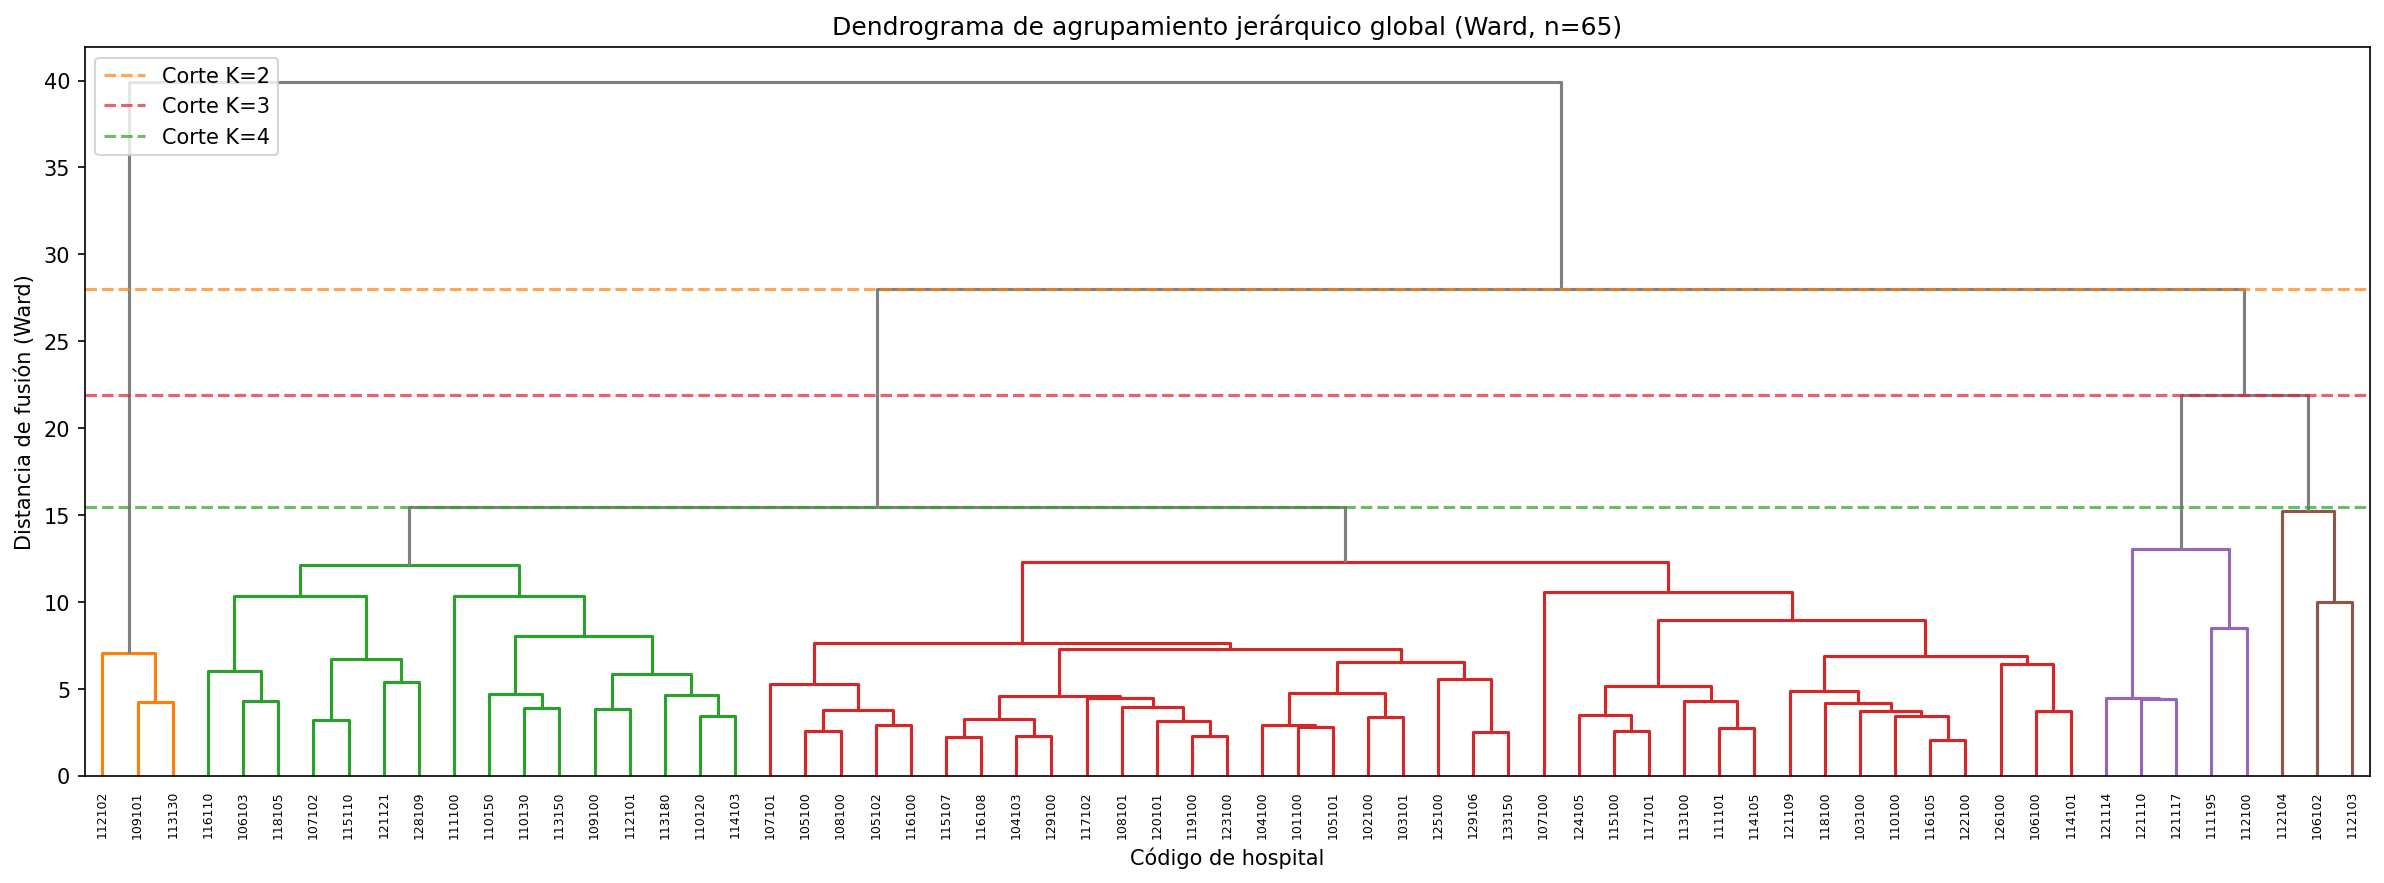
\includegraphics[width=\textwidth]{img/dendrograma_ward_nivel1.png}
\caption{Dendrograma de agrupamiento jerárquico global del Nivel 1 mediante
Ward aglomerativo. Los colores de las ramas identifican los cuatro clústeres de
la partición reportada ($K=4$). Las ramas grises corresponden a fusiones entre
clústeres. Las líneas discontinuas se ubican entre las alturas de fusión que
delimitan los cortes $K=2$, $K=3$ y $K=4$.}
\label{fig:dendrograma-global}
\end{figure}

Para caracterizar cuantitativamente los cuatro clústeres obtenidos, la
Tabla~\ref{tab:perfiles-nivel1} presenta las medianas de variables
clínico-operativas seleccionadas. Estas diferencias permiten describir los
perfiles antes de asignarles etiquetas funcionales.

\begin{table}[htbp]
\centering
\caption{Medianas de los perfiles funcionales de los clústeres del Nivel 1
($K=4$).}
\label{tab:perfiles-nivel1}
\begin{tabular}{l c c c c}
\toprule
\textbf{Variable} & \textbf{$C0$ ($n=3$)} & \textbf{$C1$ ($n=54$)} &
\textbf{$C2$ ($n=5$)} & \textbf{$C3$ ($n=3$)} \\
\midrule
Egresos por año & 7{,}115 & 13{,}124 & 4{,}627 & 4{,}038 \\
Estancia media (días) & 6{,}1 & 6{,}8 & 8{,}7 & 8{,}7 \\
Peso medio GRD & 1{,}202 & 0{,}947 & 0{,}943 & 1{,}874 \\
Entropía GRD (índice 0--1) & 0{,}789 & 0{,}821 & 0{,}832 & 0{,}775 \\
Severidad media & 1{,}949 & 1{,}666 & 1{,}908 & 1{,}892 \\
Comorbilidades promedio & 3{,}68 & 4{,}45 & 5{,}52 & 6{,}00 \\
Tasa de CMA & 13{,}5\% & 14{,}4\% & 34{,}8\% & 0{,}0\% \\
Egresos pediátricos & 95{,}4\% & 14{,}2\% & 2{,}5\% & 0{,}0\% \\
Egresos geriátricos & 0{,}0\% & 25{,}6\% & 37{,}2\% & 46{,}0\% \\
Ingresos obstétricos & 0{,}0\% & 20{,}0\% & 10{,}5\% & 0{,}0\% \\
Proporción de egresos neonatales & 0{,}0\% & 2{,}8\% & 0{,}461\% & 0{,}0\% \\
Edad mediana (años) & 5{,}0 & 41{,}8 & 56{,}8 & 63{,}6 \\
\bottomrule
\end{tabular}
\end{table}

La interpretación de los perfiles de la Tabla~\ref{tab:perfiles-nivel1} permite
caracterizar empíricamente cada grupo y, a partir de esa evidencia, derivar una
etiqueta funcional descriptiva de forma posterior al agrupamiento. El algoritmo
no recibió nombres ni categorías funcionales durante la construcción de la
partición.

\begin{itemize}
    \item \textbf{Clúster $C0$ ($n=3$): Hospitales Pediátricos.} Concentra
    prácticamente la totalidad de sus egresos en población pediátrica
    ($95{,}4\%$) y registra una edad mediana de ingreso de $5{,}0$ años, con
    actividad geriátrica y obstétrica nula. El peso medio GRD ($1{,}202$) y la
    severidad media ($1{,}949$) reflejan la complejidad de las especialidades
    infantiles. Está integrado por el Hospital Clínico de Niños Dr.\ Roberto del
    Río, el Hospital de Niños Dr.\ Luis Calvo Mackenna y el Hospital Dr.\
    Exequiel González Cortés.

    \item \textbf{Clúster $C3$ ($n=3$): grupo de especialización clínica
    heterogénea.} Registra el peso medio GRD más alto entre los cuatro perfiles
    (mediana $1{,}874$), la mayor edad mediana de la red ($63{,}6$ años), una
    estancia media de $8{,}7$ días y actividad obstétrica, pediátrica y CMA
    nula. Integra al Instituto Nacional de Enfermedades Respiratorias y Cirugía
    Torácica (INER), al Instituto de Neurocirugía Dr.\ Alfonso Asenjo y al
    Hospital Dr.\ Eduardo Pereira Ramírez de Valparaíso. Los dos primeros son
    establecimientos especializados, mientras que el tercero es un hospital
    general. Los coeficientes Silhouette individuales son $0{,}270$ para INER,
    $0{,}053$ para el Instituto de Neurocirugía y $-0{,}173$ para el Hospital
    Eduardo Pereira. Este último también cumple los tres criterios de atipicidad
    combinados (Sección~\ref{sec:res-outliers-combinados}), por lo que su
    asignación a $C3$ debe interpretarse como ambigua. En consecuencia, la
    etiqueta describe un patrón de especialización clínica del grupo, sin
    atribuir carácter monográfico al conjunto de sus tres establecimientos.

    \item \textbf{Clúster $C2$ ($n=5$): grupo de carga clínica heterogénea.}
    Comparte con $C3$ una estancia media prolongada ($8{,}7$ días) y una
    población de mayor edad (edad mediana $56{,}8$ años; $37{,}2\%$ de egresos
    geriátricos), pero su peso medio GRD ($0{,}943$) es cercano al del núcleo
    generalista. Destaca por una mediana de comorbilidades superior a la del
    núcleo ($5{,}52$ frente a $4{,}45$) y por una tasa de CMA heterogénea, cuya
    mediana es $34{,}8\%$. Está integrado por el HUAP Dr.\ Alejandro del Río,
    el Hospital Del Salvador, el Hospital Dr.\ Abraham Godoy de Lautaro, el
    Hospital Intercultural de Nueva Imperial y el Hospital de Pitrufquén.

    El grupo reúne hospitales de escala y localización distintas. Por ejemplo,
    el HUAP presenta una tasa de CMA de $0{,}1\%$, coherente con su función de
    urgencia y trauma de alta complejidad, mientras que el Hospital Dr.\ Abraham
    Godoy alcanza $41{,}6\%$. Esta heterogeneidad hace preferible mantener la
    denominación descriptiva $C2$, sin imponer una etiqueta funcional breve que
    simplifique en exceso a sus cinco integrantes.

    \item \textbf{Clúster $C1$ ($n=54$): Núcleo Generalista.} Es el grupo
    mayoritario de hospitales generales de la red pública. Presenta una mediana
    de 13.124 egresos anuales, estancia media de $6{,}8$ días, peso medio GRD de $0{,}947$ y una composición asistencial mixta, con $14{,}2\%$ de egresos pediátricos, $25{,}6\%$ de egresos geriátricos, $20{,}0\%$ de ingresos obstétricos y una proporción de egresos neonatales de $2{,}8\%$. La diversidad y el equilibrio relativo de su actividad
    permiten describirlo como el Núcleo Generalista de la red.
\end{itemize}

La proyección bidimensional mediante componentes principales de la
Figura~\ref{fig:pca-nivel1} ilustra la disposición de los hospitales en las dos
primeras componentes principales para las soluciones $K=2$, $K=3$ y $K=4$. Esta
proyección facilita examinar visualmente la separación de los establecimientos
especializados respecto del núcleo generalista, pero no constituye una prueba
adicional de validez del clustering.

\begin{figure}[htbp]
\centering
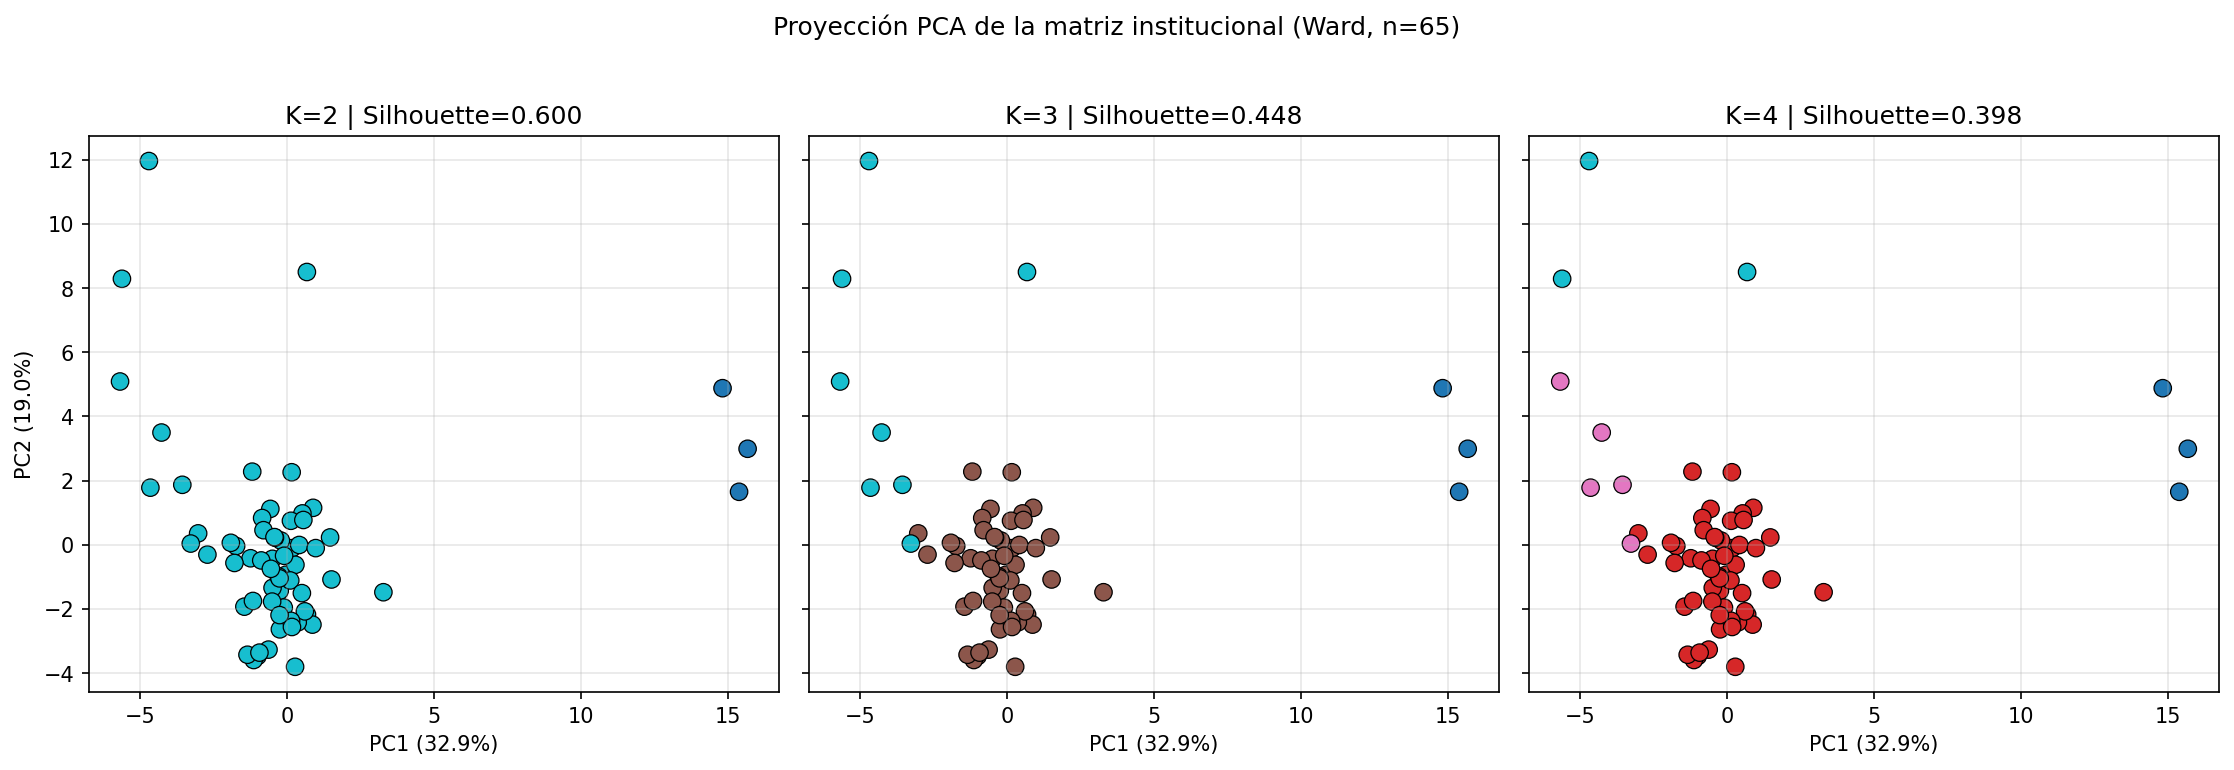
\includegraphics[width=\textwidth]{img/pca_particiones_nivel1.png}
\caption{Proyecciones bidimensionales PCA de la matriz institucional para las
soluciones Ward con $K=2$, $K=3$ y $K=4$. Los valores de Silhouette mostrados
corresponden a cada partición.}
\label{fig:pca-nivel1}
\end{figure}


\section{Subtipología exploratoria del bloque generalista (nivel 2)}
\label{sec:nivel2}

Dado que el clúster $C1$ concentra 54 de los 65 hospitales
($83{,}1\%$ del sistema), se aplicó un segundo nivel de clustering sobre este
subconjunto, de acuerdo con el diseño descrito en la
Sección~\ref{sec:nivel2-metodo}. Al operar sobre un subconjunto de hospitales,
esta subdivisión tiene un carácter exploratorio: su propósito no es establecer
fronteras funcionales equivalentes a las del Nivel~1, sino describir posibles
gradientes de volumen, complejidad y orientación clínica dentro del núcleo
generalista.

La búsqueda de configuraciones para
$K_{sub}\in\{2,3,\ldots,10\}$ se presenta en la
Tabla~\ref{tab:metricas-nivel2}. Además de las métricas internas, se reportan
los tamaños de grupo, la cantidad de grupos unitarios y el número de
subclústeres con al menos cuatro hospitales.

\begin{table}[htbp]
\centering
\caption{Búsqueda de subclústeres Ward en el núcleo generalista (Nivel~2, $n=54$).}
\label{tab:metricas-nivel2}

\begin{tabular}{c c c c c c l}
\toprule
\textbf{$K_{sub}$} & \textbf{Silhouette} & \textbf{Davies--Bouldin} & \textbf{Unitarios} & \textbf{Pares} & \textbf{$n\geq4$} & \textbf{Tamaños} \\
\midrule
2 & 0,193 & 2,303 & 0 & 0 & 2 & 40, 14 \\
3 & 0,113 & 2,282 & 0 & 0 & 3 & 29, 14, 11 \\
4 & 0,129 & 1,957 & 0 & 0 & 4 & 29, 11, 8, 6 \\
5 & 0,122 & 1,583 & 1 & 0 & 4 & 29, 10, 8, 6, 1 \\
6 & 0,132 & 1,486 & 1 & 0 & 5 & 29, 10, 6, 4, 4, 1 \\
7 & 0,136 & 1,285 & 2 & 0 & 5 & 29, 10, 5, 4, 4, 1, 1 \\
8 & 0,111 & 1,423 & 2 & 0 & 6 & 15, 14, 10, 5, 4, 4, 1, 1 \\
\textbf{9} & \textbf{0,101} & \textbf{1,368} & \textbf{2} & \textbf{0} & \textbf{7} & \textbf{15, 10, 9, 5, 5, 4, 4, 1, 1} \\
10 & 0,109 & 1,294 & 2 & 1 & 6 & 15, 10, 9, 5, 4, 4, 3, 2, 1, 1 \\
\bottomrule
\end{tabular}
\end{table}

Para evaluar si estas divisiones se reproducen al perturbar la muestra, se
aplicó al Nivel~2 el mismo protocolo de 100 submuestras sin reposición empleado
para el Nivel~1. En cada réplica se seleccionaron 43 de los 54 hospitales,
se ajustó nuevamente el preprocesamiento y se aplicó Ward. La Tabla~\ref{tab:estabilidad-nivel2}
resume la concordancia con la partición de referencia para $K_{sub}=2$, $3$ y
$9$.

\begin{table}[htbp]
\centering
\caption{Estabilidad de la partición Ward por submuestreo, Nivel~2 (100 réplicas).}
\label{tab:estabilidad-nivel2}
\begin{tabular}{c c c c}
\toprule
\textbf{$K_{sub}$} & \textbf{Silhouette original} & \textbf{ARI mediano [P2,5; P97,5]} & \textbf{NMI mediano [P2,5; P97,5]} \\
\midrule
2 & 0,193 & 0,526 [0,022; 1,000] & 0,456 [0,035; 1,000] \\
3 & 0,113 & 0,475 [0,127; 0,835] & 0,538 [0,277; 0,814] \\
9 & 0,101 & 0,559 [0,353; 0,840] & 0,774 [0,664; 0,919] \\
\bottomrule
\end{tabular}
\end{table}

La solución con dos grupos tiene el mayor Silhouette del barrido, pero su ARI
mediano de 0,526 sigue lejos de la estabilidad del Nivel~1 (ARI mediano
0,958). La solución de nueve grupos tampoco reproduce una tipología robusta:
aunque su NMI es mayor, su ARI mediano es 0,559, y contiene dos subgrupos
unitarios. En consecuencia, el Nivel~2 se limita en el cuerpo del texto a una
separación exploratoria amplia en dos bloques de 40 y 14 hospitales, por lo que no se
sostienen nueve perfiles funcionales generalizables. La asignación de nueve
subgrupos y sus perfiles descriptivos se conserva en el Anexo como material
suplementario.

Los casos $S1$ (Hospital Clínico San Borja--Arriarán) y $S8$ (Hospital Dr. Gustavo
Fricke) de la solución suplementaria son observaciones unitarias alejadas del
centroide del núcleo, no subtipos funcionales. Por tanto, no se usan para
inferencias ni para etiquetar categorías hospitalarias.

\section{Estabilidad de la partición mediante submuestreo}
\label{sec:res-estabilidad}

Siguiendo el procedimiento descrito en la Sección~\ref{sec:bootstrap}, se ejecutaron 100 iteraciones de submuestreo sin reposición. En cada réplica se seleccionó el $80\,\%$ de los 65 hospitales ($n_{\text{sub}}=52$), se recalculó el preprocesamiento y se aplicó clustering jerárquico Ward con $K=4$. La Tabla~\ref{tab:estabilidad-global} presenta los intervalos percentilares empíricos (percentiles 2{,}5 y 97{,}5) del coeficiente Silhouette de cada submuestra y de la concordancia entre su partición y la asignación original, medida mediante ARI y NMI.

\begin{table}[htbp]
\centering
\caption{Estabilidad global de la partición Ward $K=4$ por submuestreo (100 réplicas del 80\,\%).}
\label{tab:estabilidad-global}
\begin{tabular}{l c c c}
\toprule
\textbf{Métrica} & \textbf{Mediana} & \textbf{Percentil 2,5} &
\textbf{Percentil 97,5} \\
\midrule
Silhouette & 0,395 & 0,225 & 0,460 \\
ARI vs. partición original & 0,958 & 0,514 & 1,000 \\
NMI vs. partición original & 0,917 & 0,656 & 1,000 \\
\bottomrule
\end{tabular}
\end{table}

La mediana del Silhouette en las submuestras ($0{,}395$) es cercana al valor obtenido para la partición completa de 65 hospitales ($0{,}401$). Por tanto, la estructura de cohesión y separación observada en la solución principal se reproduce habitualmente al retirar una fracción de los establecimientos. No obstante, el intervalo percentilar $[0{,}225;\,0{,}460]$ muestra que la calidad interna de la partición varía entre réplicas. Algunas submuestras
producen agrupamientos menos compactos que la solución calculada sobre el conjunto completo.

La concordancia con la partición original es alta en la réplica típica, pues las medianas de ARI y NMI alcanzan $0{,}958$ y $0{,}917$, respectivamente. Sin embargo, los percentiles inferiores de ambas métricas (ARI $=0{,}514$ y NMI $=0{,}656$) indican que existen submuestras en las que la composición de los grupos se modifica en mayor medida. En consecuencia, los resultados respaldan una estructura global generalmente reproducible, pero no implican que la pertenencia de todos los hospitales a su clúster se conserve con la misma consistencia en cada submuestra.

Para localizar esta variabilidad, la Tabla~\ref{tab:estabilidad-grupo} desagrega la estabilidad por clúster mediante dos indicadores. La estabilidad individual promedio corresponde a la coasignación media de cada hospital con los demás integrantes de su clúster original, condicionada a las réplicas en que ambos hospitales fueron seleccionados. El índice de Jaccard promedio cuantifica el solapamiento entre los integrantes originales de cada clúster presentes en una submuestra y el grupo de dicha réplica con el que presentan mayor coincidencia.

\begin{table}[htbp]
\centering
\caption{Estabilidad de la partición desagregada por clúster del Nivel 1 (100 submuestras).}
\label{tab:estabilidad-grupo}
\begin{tabular}{l c c c}
\toprule
\textbf{Clúster} & \textbf{$n$} &
\textbf{Estabilidad individual (media)} &
\textbf{Jaccard promedio} \\
\midrule
$C0$ (pediátricos) & 3 & 1,000 & 1,000 \\
$C1$ (núcleo generalista) & 54 & 0,946 & 0,967 \\
$C2$ (perfil de carga clínica) & 5 & 0,967 & 0,791 \\
$C3$ (perfil monográfico) & 3 & 0,911 & 0,904 \\
\bottomrule
\end{tabular}
\end{table}

El clúster pediátrico $C0$ presenta coasignación y solapamiento perfectos en las 100 réplicas, lo que es consistente con su perfil clínico claramente diferenciado respecto del resto de la red. El núcleo generalista $C1$, que reúne 54 hospitales, también muestra una elevada estabilidad conjunta: su Jaccard promedio es $0{,}967$ y su estabilidad individual media alcanza $0{,}946$. Así, la mayor parte de los hospitales generalistas conserva su relación de proximidad con los demás integrantes del núcleo al modificar la muestra de análisis.

El clúster $C2$ registra la mayor estabilidad individual promedio entre los grupos no pediátricos ($0{,}967$), aunque su Jaccard promedio es el menor de la partición ($0{,}791$). Esto señala que sus hospitales tienden a mantener una alta coasignación con sus pares originales cuando son seleccionados, pero que la composición completa del grupo es más sensible a la omisión de algunos establecimientos en las submuestras. Esta sensibilidad es coherente con el tamaño reducido del clúster ($n=5$), pues la exclusión de uno o más de sus integrantes altera proporcionalmente su composición en mayor medida que en el núcleo generalista.

Por su parte, el clúster monográfico $C3$ presenta estabilidad individual media de $0{,}911$ y un Jaccard promedio de $0{,}904$. Ambos valores son inferiores a los observados en $C0$ y $C1$, pero no permiten caracterizar a $C3$ como un grupo inestable, pues en la mayoría de
las réplicas sus tres hospitales conservan una asociación reconocible. En conjunto, el submuestreo muestra que la partición de Nivel~1 es predominantemente reproducible, aunque la estabilidad de los grupos pequeños y la asignación de algunos establecimientos específicos dependen en mayor medida de la composición de la muestra analizada. Estos resultados constituyen evidencia de sensibilidad interna del procedimiento y deben interpretarse junto con los análisis descriptivos, de sensibilidad temporal y de detección de observaciones atípicas presentados en las secciones precedentes.


\section{Validación estadística por variable}
\label{sec:res-validacion}

Siguiendo el procedimiento descrito en la Sección~\ref{sec:validacion-grupos},
se aplicó la prueba de Kruskal-Wallis ($\alpha=0{,}05$) a las 28 variables
originales en escala no transformada. Los $p$-valores se ajustaron mediante el
procedimiento de Benjamini-Hochberg (BH), con el propósito de controlar la tasa
de falsos descubrimientos al efectuar comparaciones simultáneas. Las variables
se ordenan según su tamaño de efecto $\varepsilon^2$, calculado mediante la
Ecuación~\ref{eq:epsilon2}, el cual cuantifica la magnitud de las diferencias
entre grupos.

Entre las variables evaluadas se incluye \texttt{peso\_medio\_cma}, que se
reporta de forma descriptiva y se incorpora a esta caracterización posterior al
agrupamiento. Sin embargo, dicho indicador fue excluido de la matriz utilizada
para construir los clústeres, debido a que no es comparable en establecimientos
sin actividad CMA, como se indicó en la Sección~\ref{sec:universo}.

Estos resultados deben interpretarse como una caracterización posterior al
agrupamiento. Dado que los clústeres se construyeron a partir de estas mismas
variables, la significancia estadística no constituye una validación
independiente de la partición. En cambio, permite identificar qué variables
presentan mayores diferencias entre los perfiles resultantes y ordenar su
contribución descriptiva mediante $\varepsilon^2$.

En el Nivel~1 (Tabla~\ref{tab:kruskal-nivel1}), 26 de las 28 variables
discriminan significativamente entre los cuatro clústeres después del ajuste
BH. Los mayores tamaños de efecto corresponden a \texttt{tasa\_partos}
($\varepsilon^2=0{,}395$), \texttt{edad\_mediana}
($\varepsilon^2=0{,}377$) y \texttt{pct\_obstetrica\_ingreso}
($\varepsilon^2=0{,}345$). Estos resultados son consistentes con la separación
entre el perfil pediátrico, los establecimientos de mayor especialización y los
hospitales generalistas, particularmente respecto de la composición etaria de
los egresos y de la actividad gineco-obstétrica.

Solo \texttt{cv\_estancia} y \texttt{pabellones\_promedio} no alcanzan significancia tras el ajuste BH. Esto indica que, bajo esta comparación y nivel de corrección, no se observa evidencia suficiente de diferencias sistemáticas entre los cuatro clústeres en la variabilidad relativa de la estancia ni en el número promedio de pabellones. No implica que estas variables sean idénticas entre grupos ni que carezcan de relevancia clínica individual.

\begin{table}[htbp]
\centering
\caption{Prueba de Kruskal-Wallis con corrección Benjamini-Hochberg, Nivel~1 ($K=4$, $n=65$).}
\label{tab:kruskal-nivel1}

\begin{tabular}{l c c c c c}
\toprule
\textbf{Variable} & \textbf{$H$} & \textbf{$p$-valor} &
\textbf{$p_{\text{BH}}$} & \textbf{$\varepsilon^2$} &
\textbf{Discrimina} \\
\midrule
tasa\_partos
& 27,1 & $5{,}62 \times 10^{-6}$ & $1{,}34 \times 10^{-4}$ & 0,395 & Sí \\
edad\_mediana
& 26,0 & $9{,}58 \times 10^{-6}$ & $1{,}34 \times 10^{-4}$ & 0,377 & Sí \\
pct\_obstetrica\_ingreso
& 24,0 & $2{,}45 \times 10^{-5}$ & $2{,}29 \times 10^{-4}$ & 0,345 & Sí \\
pct\_pediatrico
& 22,9 & $4{,}16 \times 10^{-5}$ & $2{,}92 \times 10^{-4}$ & 0,327 & Sí \\
pct\_femenino\_fertil
& 22,1 & $6{,}31 \times 10^{-5}$ & $3{,}53 \times 10^{-4}$ & 0,313 & Sí \\
tasa\_prematurez
& 20,5 & $1{,}31 \times 10^{-4}$ & $6{,}13 \times 10^{-4}$ & 0,287 & Sí \\
pct\_geriatrico
& 20,2 & $1{,}56 \times 10^{-4}$ & $6{,}22 \times 10^{-4}$ & 0,282 & Sí \\
severidad\_media
& 19,4 & $2{,}31 \times 10^{-4}$ & $7{,}24 \times 10^{-4}$ & 0,268 & Sí \\
mortalidad\_media
& 19,3 & $2{,}33 \times 10^{-4}$ & $7{,}24 \times 10^{-4}$ & 0,268 & Sí \\
pct\_alta\_domicilio
& 17,1 & $6{,}64 \times 10^{-4}$ & $1{,}86 \times 10^{-3}$ & 0,232 & Sí \\
pct\_urgencia
& 16,8 & $7{,}83 \times 10^{-4}$ & $1{,}99 \times 10^{-3}$ & 0,226 & Sí \\
estancia\_mediana
& 16,3 & $9{,}79 \times 10^{-4}$ & $2{,}28 \times 10^{-3}$ & 0,218 & Sí \\
egresos\_por\_anio
& 14,1 & $0{,}003$ & $0{,}006$ & 0,182 & Sí \\
peso\_medio\_grd
& 13,6 & $0{,}004$ & $0{,}007$ & 0,173 & Sí \\
pct\_programada
& 13,4 & $0{,}004$ & $0{,}007$ & 0,170 & Sí \\
pct\_alta\_fallecido
& 13,3 & $0{,}004$ & $0{,}007$ & 0,169 & Sí \\
estancia\_media
& 13,1 & $0{,}004$ & $0{,}007$ & 0,166 & Sí \\
comorbilidades\_promedio
& 12,9 & $0{,}005$ & $0{,}007$ & 0,163 & Sí \\
pct\_uso\_pabellon
& 12,6 & $0{,}006$ & $0{,}008$ & 0,157 & Sí \\
pct\_alta\_traslado
& 12,4 & $0{,}006$ & $0{,}008$ & 0,154 & Sí \\
peso\_medio\_cma
& 12,4 & $0{,}006$ & $0{,}008$ & 0,153 & Sí \\
pct\_estancia\_larga
& 11,8 & $0{,}008$ & $0{,}010$ & 0,144 & Sí \\
pct\_origen\_referencia
& 11,3 & $0{,}010$ & $0{,}012$ & 0,137 & Sí \\
tasa\_cma
& 10,7 & $0{,}014$ & $0{,}016$ & 0,126 & Sí \\
entropia\_grd
& 9,5 & $0{,}024$ & $0{,}026$ & 0,106 & Sí \\
pct\_origen\_emergencia
& 9,4 & $0{,}024$ & $0{,}026$ & 0,105 & Sí \\
cv\_estancia
& 5,5 & $0{,}139$ & $0{,}144$ & 0,041 & No \\
pabellones\_promedio
& 4,8 & $0{,}188$ & $0{,}188$ & 0,029 & No \\
\bottomrule
\end{tabular}
\end{table}

La circularidad asociada a esta caracterización se examinó mediante dos
nulas sobre el flujo completo descritas en la
Sección~\ref{sec:permutacion-circularidad}. La primera permutó de forma
independiente cada variable entre hospitales, preservando su distribución
marginal y eliminando la estructura conjunta. En 500 repeticiones, la mediana
del número de variables significativas fue 1, el percentil 95 fue 5 y el máximo
fue 10. Ninguna réplica alcanzó las 26 variables observadas. Este resultado
muestra que Ward no genera el patrón observado cuando se eliminan por completo
las dependencias entre variables.

La segunda nula simuló 500 matrices normales multivariadas con la media y
covarianza observadas después de las transformaciones y el escalado robusto. Al
preservar la dependencia lineal, esta referencia es más exigente: la mediana
fue 23 variables significativas, el percentil 95 fue 26 y el máximo fue 28. En
59 de 500 réplicas la nula igualó o superó las 26 variables observadas
($p_{\mathrm{emp}}=0{,}1198$, con corrección de continuidad). Por tanto, el
número de diferencias detectadas por Kruskal--Wallis no supera de forma
concluyente lo esperable de una geometría correlacionada sin una estructura de
grupos explícita. La Tabla~\ref{tab:nulas-circularidad} resume los resultados de
ambas nulas. Estas pruebas mantienen utilidad descriptiva para ordenar los
atributos que difieren en la partición obtenida, pero no aportan validación
independiente de los clústeres.

\begin{table}[htbp]
\centering
\caption{Nulas del flujo Ward $K=4$ y Kruskal--Wallis/BH: número de variables significativas de 28 evaluadas.}
\label{tab:nulas-circularidad}
\begin{tabular}{l c c c c}
\toprule
\textbf{Nula} & \textbf{Mediana} & \textbf{P95} & \textbf{Máximo} & \textbf{$p_{\mathrm{emp}}$} \\
\midrule
Permutación independiente por columna & 1 & 5 & 10 & $<0{,}002$ \\
Normal multivariada con covarianza preservada & 23 & 26 & 28 & 0,1198 \\
\bottomrule
\end{tabular}
\par\smallskip
\begin{minipage}{\textwidth}
\normalsize\raggedright
\textit{Nota.} Ambas nulas usan 500 réplicas. El valor observado fue 26. En la
segunda nula, la covarianza se preserva en esperanza, con un error relativo mediano
entre la covarianza muestral simulada y la observada de 0,308.
\end{minipage}
\end{table}

En el Nivel~2 (Tabla~\ref{tab:kruskal-nivel2}), el análisis se restringe a los 54 hospitales del núcleo generalista y compara los nueve subclústeres exploratorios ($S0$ a $S8$). De las 28 variables evaluadas, 24 presentan diferencias estadísticamente detectables entre subgrupos después del ajuste BH. Las seis con mayor tamaño de efecto corresponden a \texttt{peso\_medio\_grd}, \texttt{pct\_femenino\_fertil}, \texttt{pct\_obstetrica\_ingreso}, \texttt{entropia\_grd}, \texttt{pct\_estancia\_larga} y \texttt{tasa\_prematurez}.

En consecuencia, la subtipología exploratoria diferencia principalmente gradientes de complejidad clínica, composición de la casuística, permanencia hospitalaria y orientación obstétrica. Por tratarse de un segundo nivel exploratorio construido sobre el mismo conjunto de variables, los $p_{\text{BH}}$ no constituyen evidencia independiente de categorías externas o definitivas, de modo que su utilidad es descriptiva para ordenar los atributos que distinguen los perfiles obtenidos.

\begin{table}[htbp]
\centering
\caption{Variables con mayor tamaño de efecto, Kruskal--Wallis con corrección BH, Nivel~2 ($K_{sub}=9$, $n=54$).}
\label{tab:kruskal-nivel2}

\begin{tabular}{l c c c c}
\toprule
\textbf{Variable} & \textbf{$H$} & \textbf{$p$-valor} & \textbf{$p_{\text{BH}}$} & \textbf{$\varepsilon^2$} \\
\midrule
peso\_medio\_grd & 41,897 & $1{,}4158 \times 10^{-6}$ & $3{,}9642 \times 10^{-5}$ & 0,75327 \\
pct\_femenino\_fertil & 37,218 & $1{,}0493 \times 10^{-5}$ & 0,00014691 & 0,64929 \\
pct\_obstetrica\_ingreso & 35,751 & $1{,}9505 \times 10^{-5}$ & 0,00016808 & 0,61668 \\
entropia\_grd & 35,256 & $2{,}4011 \times 10^{-5}$ & 0,00016808 & 0,60570 \\
pct\_estancia\_larga & 34,309 & $3{,}5715 \times 10^{-5}$ & 0,00019920 & 0,58464 \\
tasa\_prematurez & 33,881 & $4{,}2686 \times 10^{-5}$ & 0,00019920 & 0,57514 \\
\bottomrule
\end{tabular}
\par\smallskip
\begin{minipage}{\textwidth}
\normalsize\raggedright
\textit{Nota.} Resultados ordenados de forma descendente por $\varepsilon^2$. La prueba caracteriza descriptivamente una partición exploratoria del Nivel~2 y no valida de forma independiente los subclústeres.
\end{minipage}
\end{table}

La magnitud de los tamaños de efecto debe considerarse junto con la significancia. Las seis variables resumidas en la Tabla~\ref{tab:kruskal-nivel2} son las que muestran las diferencias relativas más intensas entre los subgrupos. Este ordenamiento, sin embargo, no implica que las fronteras entre ellos sean robustas o generalizables.

Adicionalmente, se examinó la asociación entre la asignación de clústeres y la pertenencia a Servicios de Salud mediante una prueba de chi-cuadrado de independencia. En el Nivel~1 se obtuvo $\chi^2=65{,}329$ ($\text{gl}=84$, $p=0{,}935$), mientras que en el Nivel~2 se obtuvo $\chi^2=206{,}944$ ($\text{gl}=224$, $p=0{,}787$). En ambos niveles no se detectó una asociación estadísticamente significativa entre los clústeres y el Servicio de Salud.

Estas tablas de contingencia son dispersas, pues relacionan un número reducido de hospitales con numerosas categorías territoriales y administrativas. En consecuencia, el V de Cramér sin corrección puede sobreestimar la
asociación. Sus valores alcanzan $0{,}579$ en el Nivel~1 y $0{,}692$
en el Nivel~2. Al aplicar la corrección de sesgo de \citet{Bergsma2013}, el V de Cramér es aproximadamente cero en ambos niveles. Por ello, bajo esta especificación no se observa una asociación apreciable entre los clústeres y los Servicios de Salud. Este resultado no permite descartar de forma concluyente toda influencia territorial o administrativa, pero no aporta evidencia de que la segmentación obtenida esté determinada por dicha pertenencia.

\section{Comparación con la clasificación MINSAL}
\label{sec:res-minsal}

Siguiendo el procedimiento de contraste descrito en la
Sección~\ref{sec:contraste-minsal}, se comparó la partición de Nivel~1
($K=4$) con las categorías administrativas de complejidad del MINSAL
(Alta y Mediana Complejidad). La Tabla~\ref{tab:contingencia-minsal}
presenta la distribución de los 65 hospitales entre ambas clasificaciones.

\begin{table}[htbp]
\centering
\caption{Tabla de contingencia entre los clústeres del Nivel~1 y la clasificación administrativa MINSAL.}
\label{tab:contingencia-minsal}
\begin{tabular}{l c c c}
\toprule
\textbf{Clúster} & \textbf{Alta Complejidad} &
\textbf{Mediana Complejidad} & \textbf{Total} \\
\midrule
$C0$ (pediátricos) & 3 & 0 & 3 \\
$C1$ (núcleo generalista) & 47 & 7 & 54 \\
$C2$ (perfil de carga clínica) & 2 & 3 & 5 \\
$C3$ (especialización clínica heterogénea) & 3 & 0 & 3 \\
\bottomrule
\end{tabular}
\end{table}

Los índices globales de concordancia entre ambas particiones alcanzan un
Índice de Rand Ajustado (ARI) de $0{,}112$ y una Información Mutua
Normalizada (NMI) de $0{,}107$. Estos valores indican una concordancia global
baja entre la clasificación administrativa y la segmentación funcional
obtenida a partir de los egresos hospitalarios. Esta diferencia es consistente
con que ambas clasificaciones organizan los establecimientos mediante criterios
distintos. La clasificación MINSAL constituye una referencia administrativa,
mientras que los clústeres de este estudio se construyen a partir de la
producción, la complejidad clínica y la composición de la casuística observada
en los egresos.

La contingencia permite precisar cómo se distribuyen los perfiles funcionales
respecto de las categorías administrativas. Los tres hospitales pediátricos de
$C0$ y los tres establecimientos del grupo de especialización clínica
heterogénea $C3$ están clasificados por MINSAL como de Alta Complejidad. Esta
coincidencia describe la ubicación administrativa de los perfiles más
especializados identificados en el Nivel~1, sin constituir una validación externa
de la partición.

El núcleo generalista $C1$ concentra 47 hospitales de Alta Complejidad y 7 de
Mediana Complejidad. Por tanto, este perfil funcional reúne establecimientos
pertenecientes a ambas categorías administrativas, aunque predomina la Alta
Complejidad. De manera complementaria, el perfil de carga clínica $C2$ incluye
dos hospitales clasificados como de Alta Complejidad y tres como de Mediana
Complejidad. En consecuencia, ninguno de estos dos perfiles funcionales se
corresponde de manera exclusiva con una categoría administrativa MINSAL.

En conjunto, el contraste muestra que la clasificación administrativa no se
reproduce directamente al agrupar hospitales según sus características de
actividad clínica y casuística. Este resultado no permite establecer la
superioridad de una clasificación sobre la otra ni atribuir la diferencia a una
causa única. Más bien, evidencia que ambas particiones aportan lecturas
distintas y complementarias sobre la red hospitalaria pública.

\subsection{Comparación directa de homogeneidad interna}
\label{sec:res-homogeneidad}

El ARI y el NMI indican cuánto concuerdan dos particiones, pero no informan
directamente sobre su homogeneidad interna. Para comparar la compactación de los
grupos, se siguió el procedimiento descrito en la
Sección~\ref{sec:comparacion-homogeneidad}. El coeficiente Silhouette y la
dispersión intragrupo normalizada (WSS/TSS) se calcularon sobre la misma matriz
preprocesada de 35 variables empleada en el clustering. De forma
complementaria, la dispersión robusta se resumió mediante la desviación absoluta
mediana normalizada (MAD normalizado) sobre las 27 variables
clínico-operativas directas.

La Tabla~\ref{tab:homogeneidad-no-controlada} compara la solución Ward $K=4$
utilizada en este trabajo con la clasificación MINSAL. Un menor WSS/TSS y un
menor MAD normalizado indican menor dispersión dentro de los grupos.

\begin{table}[htbp]
\centering
\caption{Comparación de homogeneidad interna no controlada por número de grupos entre Ward $K=4$ y MINSAL.}
\label{tab:homogeneidad-no-controlada}
\begin{tabular}{l c c c c c}
\toprule
\textbf{Partición} & \textbf{$K$} & \textbf{Tamaños} &
\textbf{Silhouette} & \textbf{WSS/TSS} &
\textbf{MAD norm.} \\
\midrule
Ward $K=4$ & 4 & 3, 54, 5, 3 & 0,401 & 0,475 & 0,895 \\
MINSAL & 2 & 55, 10 & 0,070 & 0,944 & 0,999 \\
\bottomrule
\end{tabular}
\end{table}

En esta comparación no controlada, Ward $K=4$ presenta menor dispersión
intragrupo que MINSAL en las tres métricas. Sin embargo, esta primera
comparación debe interpretarse considerando que Ward utiliza cuatro grupos,
mientras que MINSAL contiene dos categorías. La fragmentación en un número
mayor de grupos puede reducir mecánicamente la dispersión intragrupo.

Por ello, la Tabla~\ref{tab:homogeneidad-controlada} repite el contraste con
Ward restringido a $K=2$, el mismo número de grupos de la clasificación MINSAL.
Ambas particiones se evalúan sobre la misma matriz y con las mismas métricas.

\begin{table}[htbp]
\centering
\caption{Comparación de homogeneidad interna controlada por número de grupos: Ward $K=2$ y MINSAL ($K=2$).}
\label{tab:homogeneidad-controlada}
\begin{tabular}{l c c c c c}
\toprule
\textbf{Partición} & \textbf{$K$} & \textbf{Tamaños} &
\textbf{Silhouette} & \textbf{WSS/TSS} &
\textbf{MAD norm.} \\
\midrule
Ward $K=2$ & 2 & 3, 62 & 0,605 & 0,707 & 0,931 \\
MINSAL & 2 & 55, 10 & 0,070 & 0,944 & 0,999 \\
\bottomrule
\end{tabular}
\end{table}

Incluso al fijar el número de grupos en $K=2$, la solución Ward presenta una
dispersión intragrupo menor que MINSAL y un Silhouette más alto. En este espacio
funcional, la separación entre los tres hospitales pediátricos y los 62
establecimientos restantes produce grupos más compactos que la partición
administrativa entre Alta y Mediana Complejidad.

La prueba de permutación evaluó si la dispersión intragrupo observada era menor
que la esperable bajo asignaciones aleatorias que preservan los tamaños de cada
partición. Se generaron 2.000 permutaciones para Ward $K=4$, Ward $K=2$ y
MINSAL. La Tabla~\ref{tab:permutacion-homogeneidad} resume los resultados.

\begin{table}[htbp]
\centering
\caption{Prueba de permutación de la dispersión intragrupo normalizada (2.000 reasignaciones).}
\label{tab:permutacion-homogeneidad}
\begin{tabular}{l c c c}
\toprule
\textbf{Partición} & \textbf{WSS/TSS observado} &
\textbf{$z$-score} & \textbf{$p$-valor empírico} \\
\midrule
Ward $K=4$ & 0,475 & $-20{,}97$ & $<0{,}001$ \\
Ward $K=2$ & 0,707 & $-20{,}98$ & $<0{,}001$ \\
MINSAL & 0,944 & $-4{,}68$ & 0,003 \\
\bottomrule
\end{tabular}
\par\smallskip
\begin{minipage}{\textwidth}
\normalsize\raggedright
\textit{Nota metodológica.} La distribución nula de WSS/TSS para MINSAL es marcadamente asimétrica (sesgo positivo): la mayor parte de las 2.000 permutaciones produce dispersiones intragrupo elevadas, con una cola derecha extendida. Esta asimetría es esperable en particiones muy desbalanceadas (grupos de 55 y 10 hospitales), donde la asignación aleatoria rara vez genera subconjuntos tan compactos como los observados. El $z$-score de $-4{,}68$ se calcula respecto de la media y desviación estándar de la distribución nula y no presupone normalidad, mientras que el $p$-valor empírico de $0{,}003$ indica que aproximadamente 6 de las 2.000 reasignaciones alcanzaron una dispersión igual o menor que la observada (WSS/TSS $= 0{,}944$). Este resultado confirma que la clasificación MINSAL presenta una compactación estadísticamente superior a la esperable por azar bajo sus propios tamaños de grupo, aunque notoriamente menor que la de las soluciones Ward.
\end{minipage}
\end{table}


Ninguna de las 2.000 particiones aleatorias para Ward $K=4$ o Ward $K=2$
alcanzó una dispersión intragrupo igual o menor que la observada. La
clasificación MINSAL también presenta una dispersión menor que la esperable bajo
asignaciones aleatorias con sus mismos tamaños de grupo, aunque con una
distancia menor respecto de su distribución nula.

Estos resultados describen la compactación interna de las particiones sobre la
matriz funcional completa. Sin embargo, Ward fue ajustado en ese mismo espacio,
por lo que sus menores valores de dispersión no constituyen una prueba
confirmatoria de mayor homogeneidad frente a MINSAL. La comparación se conserva
como diagnóstico descriptivo y se complementa a continuación con una evaluación
en bloques de variables no usados para construir las etiquetas Ward.

\subsection{Validación cruzada por bloques de variables}
\label{sec:res-homogeneidad-cruzada}

La Tabla~\ref{tab:homogeneidad-cruzada} evalúa cada partición en un bloque de
variables distinto del que se utilizó para construir Ward. Al agrupar con las 27
variables directas y evaluar sobre las 8 componentes de casuística, Ward $K=4$
obtuvo WSS/TSS $=0{,}616$, frente a $0{,}956$ para MINSAL, con una diferencia
MINSAL--Ward de $0{,}340$ (IC bootstrap 95\,\% $[0{,}176;0{,}540]$). En el
sentido inverso, al agrupar con componentes de casuística y evaluar sobre las
variables directas, Ward $K=4$ obtuvo WSS/TSS $=0{,}533$, frente a $0{,}940$
para MINSAL, con una diferencia de $0{,}407$ (IC 95\,\%
$[0{,}198;0{,}616]$). En ambas direcciones, la partición de cuatro grupos
conserva menor dispersión en el bloque retenido.

\begin{table}[htbp]
\centering
\caption{Validación cruzada de homogeneidad por bloques de variables. Ward se
ajusta solo en el bloque de agrupamiento y ambas particiones se evalúan en el
bloque retenido. La diferencia es $\mathrm{WSS/TSS}_{\mathrm{MINSAL}}-
\mathrm{WSS/TSS}_{\mathrm{Ward}}$; valores positivos favorecen menor dispersión
para Ward.}
\label{tab:homogeneidad-cruzada}

\begin{tabular}{l c c c c}
\toprule
\textbf{Bloque de agrupamiento} & \textbf{$K$ Ward} &
\textbf{WSS/TSS Ward} & \textbf{WSS/TSS MINSAL} &
\textbf{Diferencia (IC 95\,\%)} \\
\midrule
Directas $\rightarrow$ casuística & 4 & 0,616 & 0,956 &
0,340 $[0,176;0,540]$ \\
Casuística $\rightarrow$ directas & 4 & 0,533 & 0,940 &
0,407 $[0,198;0,616]$ \\
\addlinespace
Directas $\rightarrow$ casuística & 2 & 0,850 & 0,956 &
0,106 $[-0,057;0,262]$ \\
Casuística $\rightarrow$ directas & 2 & 0,740 & 0,940 &
0,200 $[-0,073;0,449]$ \\
\bottomrule
\end{tabular}
\par\smallskip
\begin{minipage}{\textwidth}
\normalsize\raggedright
\textit{Nota.} Los intervalos se obtuvieron mediante 5.000 remuestreos de los
65 hospitales. La evaluación cruzada por bloques no es independiente en sentido
temporal: ambos bloques derivan de los mismos establecimientos y período.
\end{minipage}
\end{table}

Al restringir Ward a $K=2$, para igualar el número de categorías de MINSAL, las
diferencias puntuales continúan siendo favorables a Ward, pero sus intervalos
bootstrap incluyen cero en ambas direcciones. Por tanto, esta evaluación no
entrega evidencia robusta de que Ward sea más homogéneo que MINSAL cuando se
controla simultáneamente la reutilización del espacio de evaluación y el número
de grupos. El resultado más acotado es que la solución Ward $K=4$ conserva una
compactación mayor en bloques retenidos, aunque parte de esa diferencia puede
asociarse a su mayor granularidad. En consecuencia, el estudio no establece una
superioridad general de la clasificación funcional sobre la administrativa, aunque sí
documenta que ambas organizan de manera distinta la actividad hospitalaria y que
los perfiles Ward muestran cohesión interna y estabilidad bajo las sensibilidades
reportadas.

\subsection{Discusión de los resultados frente a antecedentes nacionales e internacionales}
\label{sec:discusion-literatura}

La baja cohesión de la clasificación MINSAL observada en esta muestra es
congruente con la evidencia nacional previa. \citet{Giglio2021} reportaron
valores de Silhouette inferiores a $0{,}2$ para esa clasificación en los años
2014--2018, con casos negativos en algunos períodos. En este estudio, evaluada
sobre una matriz distinta, construida con registros GRD de 2019--2024 y solo con
hospitales de alta y mediana complejidad, la partición MINSAL alcanzó un
Silhouette de $0{,}070$. Los valores no son directamente intercambiables por las
diferencias de universo, período y variables, pero su coincidencia cualitativa
refuerza la conclusión acotada de que las etiquetas administrativas no capturan
por sí solas una estructura compacta de actividad clínica y casuística.

Los resultados también actualizan y matizan el hallazgo de \citet{Carlier2020},
quienes identificaron a la categoría de mediana complejidad como la menos
consistente entre años al intentar reproducir la clasificación administrativa
mediante indicadores de producción. En la presente partición, siete de los diez
hospitales MINSAL de mediana complejidad se integran al núcleo generalista $C1$,
junto con 47 hospitales de alta complejidad, los tres restantes se ubican en el
grupo $C2$, que también contiene dos hospitales de alta complejidad. Esta
distribución indica que las categorías administrativas no se corresponden de
forma exclusiva con los perfiles funcionales identificados. Sin embargo, no
permite atribuir la discrepancia a una categoría administrativa particular ni
comparar directamente la estabilidad temporal de ambos estudios, ya que sus
datos, variables y procedimientos de agrupamiento son distintos.

La comparación con el estudio francés de \citet{Chrusciel2021} muestra, a su
vez, que los ejes de organización funcional dependen de la información incluida
y del contexto de red. Ese trabajo identificó tres grupos principalmente
asociados con tamaño, diversidad y movilidad de pacientes. En esta tesis, la
solución de cuatro grupos distingue un núcleo generalista y perfiles pediátrico,
monográfico y de carga clínica heterogénea. La composición
demográfico-obstétrica aporta el $37{,}1\,\%$ de la distancia total, aunque la
partición se conserva en gran medida al excluir ese bloque ($ARI=0{,}933$).
Por tanto, la estructura chilena estudiada no se explica solo por la composición
de la demanda, pero esta dimensión participa más explícitamente que en el diseño
francés. La diferencia no contradice el antecedente internacional, ilustra que
las tipologías obtenidas son sensibles a las variables disponibles y que no
corresponde trasladar un número de grupos ni etiquetas funcionales entre redes
sin una evaluación contextual.

En conjunto, los tres antecedentes sitúan el aporte de esta investigación como una
actualización reproducible de la caracterización funcional de hospitales
chilenos con datos GRD recientes. La evidencia respalda la utilidad descriptiva
de complementar las categorías administrativas con información de producción y
casuística, pero no valida una tipología universal ni justifica usar la
partición Ward como criterio único para decisiones de financiamiento, desempeño
o asignación de recursos.

\subsection{Regresión LASSO: variables clínicas asociadas a la etiqueta MINSAL}
\label{sec:res-lasso}

El contraste anterior cuantifica la concordancia y la homogeneidad interna de
las particiones, pero no identifica qué variables de actividad clínica se
asocian con la clasificación administrativa. Para explorar esta relación, se
ajustó una regresión logística LASSO con penalización $L_1$ ($C=0{,}5$). La
variable objetivo fue el Nivel de Complejidad MINSAL, codificado como Alta
Complejidad $=1$ y Mediana Complejidad $=0$.

El modelo utilizó 27 variables clínico-operativas directas sobre los 65
hospitales, excluyendo las ocho componentes PCA de casuística y el indicador
\texttt{peso\_medio\_cma}. Esta exclusión mantiene la consistencia con la
matriz de clustering, pues \texttt{peso\_medio\_cma} no es comparable cuando un
establecimiento no registra actividad CMA.

La selección se evaluó mediante validación cruzada estratificada de cinco
pliegues. El procedimiento retuvo un máximo de ocho variables con mayor
frecuencia de selección. La Tabla~\ref{tab:lasso-frecuencia} presenta las ocho
variables retenidas y sus coeficientes en el modelo final ajustado sobre la
muestra completa.

\begin{table}[htbp]
\centering
\caption{Variables retenidas por LASSO: frecuencia de selección y coeficiente del modelo final.}
\label{tab:lasso-frecuencia}
\begin{tabular}{l c c}
\toprule
\textbf{Variable} & \textbf{Frecuencia de selección} &
\textbf{Coeficiente final} \\
\midrule
egresos\_por\_anio & 1,00 & 1,566 \\
pct\_estancia\_larga & 1,00 & 0,267 \\
pct\_alta\_traslado & 1,00 & $-0{,}567$ \\
pct\_femenino\_fertil & 0,80 & $-0{,}382$ \\
pct\_uso\_pabellon & 0,80 & 0,281 \\
tasa\_prematurez & 0,60 & 0,040 \\
cv\_estancia & 0,60 & 0,075 \\
comorbilidades\_promedio & 0,60 & $-0{,}103$ \\
\bottomrule
\end{tabular}
\end{table}

Las tres variables seleccionadas en todos los pliegues fueron
\texttt{egresos\_por\_anio}, \texttt{pct\_estancia\_larga} y
\texttt{pct\_alta\_traslado}. En el modelo final, \texttt{egresos\_por\_anio}
presenta el coeficiente estandarizado de mayor magnitud positiva. Dentro de este
modelo y esta muestra, un mayor volumen anual de egresos se asocia con una mayor
probabilidad estimada de pertenecer a la categoría de Alta Complejidad MINSAL.

Las demás variables retenidas muestran asociaciones condicionales de menor
magnitud. El signo negativo de \texttt{pct\_alta\_traslado} indica que, al
controlar por las demás variables del modelo, una mayor proporción de traslados
se asocia con una menor probabilidad estimada de Alta Complejidad. Estos
coeficientes describen asociaciones predictivas dentro de la muestra y no deben
interpretarse como efectos causales ni como criterios utilizados directamente
por MINSAL para asignar sus categorías.

Nueve variables alcanzaron una frecuencia de selección igual o superior a
$0{,}60$. Sin embargo, el procedimiento limita la selección a ocho variables,
por lo que \texttt{peso\_medio\_grd}, también seleccionado en tres de los cinco
pliegues, no fue retenido dentro del máximo establecido. Esta restricción evita
incrementar el número de predictores en una muestra con solo 65 hospitales.

El desempeño predictivo se evaluó fuera de muestra mediante la misma validación
cruzada estratificada de cinco pliegues. La Tabla~\ref{tab:lasso-desempeno}
presenta los resultados por pliegue.

\begin{table}[htbp]
\centering
\caption{Desempeño fuera de muestra del modelo LASSO (validación cruzada estratificada, 5 pliegues).}
\label{tab:lasso-desempeno}
\begin{tabular}{c c c c}
\toprule
\textbf{Pliegue} & \textbf{$n$ de prueba} &
\textbf{Accuracy} & \textbf{AUC} \\
\midrule
0 & 13 & 0,846 & 1,000 \\
1 & 13 & 0,846 & 1,000 \\
2 & 13 & 0,923 & 1,000 \\
3 & 13 & 1,000 & 1,000 \\
4 & 13 & 0,846 & 0,909 \\
\midrule
Promedio & -- & 0,892 & 0,982 \\
Baseline de clase mayoritaria & -- & 0,846 & -- \\
\bottomrule
\end{tabular}
\end{table}

La exactitud media del modelo alcanza $0{,}892$, mientras que un clasificador
que asignara siempre la categoría mayoritaria alcanzaría $0{,}846$. El AUC
medio es $0{,}982$. Estos resultados indican que las variables incluidas en el
modelo contienen información para discriminar, dentro de esta muestra, entre
las categorías administrativas de Alta y Mediana Complejidad.

Sin embargo, la interpretación debe reconocer el tamaño reducido y el
desbalance de la clase minoritaria. Solo 10 hospitales pertenecen a la categoría
de Mediana Complejidad, de modo que cada pliegue de prueba contiene dos
establecimientos de esa categoría. Por ello, las métricas de validación cruzada
deben leerse como evidencia exploratoria de capacidad discriminante y no como
una estimación definitiva del desempeño en otras poblaciones hospitalarias.

En conjunto, la regresión LASSO complementa la baja concordancia global entre la
segmentación funcional y MINSAL. El análisis identifica un conjunto reducido de
variables de actividad asociadas a la etiqueta administrativa en esta muestra,
entre las cuales el volumen anual de egresos presenta la asociación positiva de
mayor magnitud. Esto no implica que la clasificación MINSAL dependa únicamente
del volumen ni que sea insensible a otros atributos institucionales. Más bien,
muestra que la clasificación administrativa y la segmentación funcional basada
en casuística describen dimensiones relacionadas, pero no equivalentes, de la
red hospitalaria.


\section{Hospitales atípicos}

\label{sec:res-outliers}

\subsection{Influencia de las marcas globales antes del clustering}
\label{sec:res-outliers-preclustering}

Como prueba de sensibilidad previa, Isolation Forest se ajustó globalmente
sobre los 65 hospitales antes de construir Ward. Con contaminación $=10\,\%$
marcó siete establecimientos. Al excluirlos temporalmente y re-estimar Ward
$K=4$ sobre los 58 restantes, el Silhouette disminuyó de $0{,}401$ a $0{,}181$
y la concordancia con la partición base, restringida a los hospitales retenidos,
fue baja ($ARI=0{,}265$; $NMI=0{,}506$). Al reasignar las siete marcas al
centroide más próximo de la solución entrenada sin ellas, la concordancia sobre
los 65 hospitales se mantuvo baja ($ARI=0{,}317$; $NMI=0{,}500$) y el
Silhouette fue $0{,}154$.

Las marcas incluyen dos hospitales pediátricos, los tres miembros del grupo
$C3$ y dos hospitales de $C2$. Por tanto, la exclusión no elimina ruido aislado:
retira perfiles especializados que participan en la estructura que el análisis
pretende describir. La solución sin marcas fragmenta el núcleo en grupos de 16
y 38 hospitales y produce un grupo unitario. En consecuencia, la partición
principal conserva los 65 establecimientos. Isolation Forest se interpreta como
una señal de influencia global y no como un criterio de eliminación automática, por lo que
los criterios posteriores permiten caracterizar con mayor detalle los casos
alejados o con asignación ambigua.

\subsection{Sensibilidad al parámetro de contaminación de Isolation Forest}

\label{sec:res-outliers-sensibilidad}

Como se indicó en la Sección~\ref{sec:outliers-metodo}, el parámetro de contaminación de Isolation Forest determina la proporción aproximada de observaciones que el algoritmo tratará como potencialmente atípicas. Por ello, con contaminación $=10\,\%$ y un universo de 65 hospitales, se espera que el modelo marque aproximadamente entre 6 y 7 establecimientos. Este resultado depende parcialmente de la configuración seleccionada y no debe interpretarse, por sí solo, como una estimación independiente de la cantidad de hospitales atípicos en la red.

Para examinar esta dependencia, se ajustó Isolation Forest globalmente sobre los 65 hospitales y las 35 variables de la matriz institucional, utilizando niveles de contaminación de $5\,\%$, $10\,\%$, $15\,\%$ y $20\,\%$. La Tabla~\ref{tab:sensibilidad-contaminacion} presenta el número objetivo aproximado y el número de hospitales efectivamente marcados en cada configuración.

\begin{table}[htbp]
\centering
\caption{Sensibilidad de Isolation Forest, ajustado globalmente, al parámetro de contaminación.}
\label{tab:sensibilidad-contaminacion}
\begin{tabular}{c c c}
\toprule
\textbf{Contaminación} & \textbf{$n$ objetivo aproximado} & \textbf{$n$ marcado} \\
\midrule
5\,\%  & 3  & 4 \\
10\,\% & 6  & 7 \\
15\,\% & 10 & 10 \\
20\,\% & 13 & 13 \\
\bottomrule
\end{tabular}
\end{table}

El número de hospitales marcados aumenta al incrementar el parámetro de contaminación, en concordancia con el funcionamiento esperado del algoritmo. En consecuencia, la configuración con contaminación $=10\,\%$ se utiliza como una elección operativa para integrar los criterios de detección, y no como un umbral determinado exclusivamente por la estructura de los datos.

Cuatro establecimientos fueron marcados en los cuatro niveles de contaminación explorados: el Hospital Dr.\ Eduardo Pereira Ramírez, el Instituto Nacional de Enfermedades Respiratorias y Cirugía Torácica, el Instituto de Neurocirugía Dr.\ Alfonso Asenjo y el Hospital Dr.\ Exequiel González Cortés. Esta persistencia indica que dichos hospitales fueron identificados de forma consistente por Isolation Forest dentro del rango de parámetros evaluado. Sin embargo, no permite establecer por sí sola la naturaleza ni la causa de sus diferencias respecto de la red hospitalaria analizada.

\subsection{Criterios combinados y detección concordante}

\label{sec:res-outliers-combinados}

La detección combinó los tres criterios descritos en la Sección~\ref{sec:outliers-metodo}: Isolation Forest ajustado globalmente con contaminación $=10\,\%$, distancia al centroide del clúster normalizada mediante la MAD global y Silhouette individual negativo. Se consideraron como casos de detección concordante los hospitales que cumplieron al menos dos de estos criterios.

La Tabla~\ref{tab:outliers} presenta los nueve hospitales marcados por al menos un criterio. Tres de ellos cumplen dos o más criterios: el Hospital Dr.\ Eduardo Pereira Ramírez, el Instituto de Neurocirugía Dr.\ Alfonso Asenjo y el Hospital de Urgencia Asistencia Pública Dr.\ Alejandro del Río. Los seis establecimientos restantes fueron identificados por una sola medida, por lo que su señalamiento depende de ese criterio particular.

\begin{table}[htbp]
\centering
\caption{Hospitales marcados por al menos un criterio de detección de atipicidad.}
\label{tab:outliers}
\par\smallskip
\begin{minipage}{\textwidth}
\normalsize\raggedright
\textit{Nota.} Los establecimientos en negrita cumplen dos o más criterios de detección.
\end{minipage}

\renewcommand{\arraystretch}{1.15}
\begin{tabular}{p{5.4cm} c c p{5.3cm}}
\toprule
\textbf{Establecimiento} & \textbf{Clúster} & \textbf{$n$} & \textbf{Criterio(s)} \\
\midrule

\textbf{Hospital Dr.\ Eduardo Pereira Ramírez}
& $C3$ & 3 &
\textbf{Isolation Forest; distancia al centroide ($z_{\mathrm{MAD}}=3{,}316$); Silhouette $=-0{,}173$} \\

\textbf{Instituto de Neurocirugía Dr.\ Alfonso Asenjo}
& $C3$ & 3 &
\textbf{Isolation Forest; distancia al centroide ($z_{\mathrm{MAD}}=3{,}905$)} \\

\textbf{Hospital de Urgencia Asistencia Pública Dr.\ Alejandro del Río}
& $C2$ & 5 &
\textbf{Isolation Forest; distancia al centroide ($z_{\mathrm{MAD}}=3{,}257$)} \\

Instituto Nacional de Enfermedades Respiratorias y Cirugía Torácica
& $C3$ & 3 &
Isolation Forest \\

Hospital Dr.\ Exequiel González Cortés
& $C0$ & 3 &
Isolation Forest \\

Hospital de Niños Dr.\ Luis Calvo Mackenna
& $C0$ & 3 &
Isolation Forest \\

Hospital del Salvador
& $C2$ & 5 &
Isolation Forest \\

Hospital Clínico San Borja-Arriarán
& $C1$ & 54 &
Distancia al centroide ($z_{\mathrm{MAD}}=3{,}281$) \\

Hospital Dr.\ Gustavo Fricke
& $C1$ & 54 &
Distancia al centroide ($z_{\mathrm{MAD}}=3{,}232$) \\

\bottomrule
\end{tabular}
\end{table}

Isolation Forest se ajustó una sola vez sobre la totalidad de los 65 hospitales. Por tanto, sus marcas indican que un establecimiento resulta relativamente aislable respecto de la red completa en el espacio de 35 variables utilizado, y no que sea necesariamente atípico dentro de su propio clúster. En cambio, la distancia al centroide evalúa el alejamiento respecto del centroide del grupo asignado, aunque su estandarización se realizó mediante la dispersión global de las distancias. El Silhouette individual resume la coherencia relativa entre la asignación del hospital a su grupo y su proximidad a los demás grupos.

El Hospital Dr.\ Eduardo Pereira Ramírez es el único establecimiento que reúne los tres criterios y que, además, presenta Silhouette individual negativo. Esto indica que su perfil se aleja del centroide de $C3$, es identificado por Isolation Forest respecto de la red global y presenta una asignación menos coherente que la del resto de los hospitales según esta medida. El Instituto de Neurocirugía Dr.\ Alfonso Asenjo y el HUAP Dr.\ Alejandro del Río cumplen los criterios de Isolation Forest y distancia al centroide, pero mantienen valores positivos de Silhouette individual.

Los resultados de Isolation Forest también incluyen establecimientos pediátricos e institutos especializados, como el Hospital Dr.\ Exequiel González Cortés, el Hospital de Niños Dr.\ Luis Calvo Mackenna y el Instituto Nacional de Enfermedades Respiratorias y Cirugía Torácica. Dado que este algoritmo compara cada hospital con la red completa, estas detecciones son compatibles con perfiles funcionales menos frecuentes dentro del conjunto analizado. No obstante, la detección estadística no permite atribuir por sí sola las diferencias a causas institucionales, clínicas, administrativas o de registro específicas.

Finalmente, el Hospital Clínico San Borja-Arriarán y el Hospital Dr.\ Gustavo Fricke fueron identificados únicamente por su distancia al centroide dentro del núcleo generalista $C1$. Ambos superan el umbral de distancia robusta definido mediante la MAD global, aunque no fueron señalados por Isolation Forest ni presentan Silhouette negativo. Por ello, su resultado describe un mayor alejamiento relativo respecto del centroide de su grupo, sin constituir evidencia suficiente para caracterizarlos como anomalías institucionales.

En conjunto, este análisis identifica establecimientos cuya posición difiere de la observada en la mayor parte de la red o de su grupo asignado. Estas marcas se emplean como una caracterización descriptiva posterior al agrupamiento y no como un juicio sobre desempeño, calidad de atención, consistencia de los registros o pertinencia administrativa de cada establecimiento.

La Figura~\ref{fig:outliers-pca} presenta una proyección bidimensional mediante PCA de los 65 establecimientos. Los círculos rojos identifican los nueve hospitales marcados por al menos uno de los criterios descritos previamente. Esta representación permite ubicar visualmente dichos establecimientos respecto de la partición Ward de Nivel~1, pero no constituye una validación independiente del agrupamiento, pues resume en dos componentes un espacio construido a partir de 35 variables.

\begin{figure}[htbp]
\centering
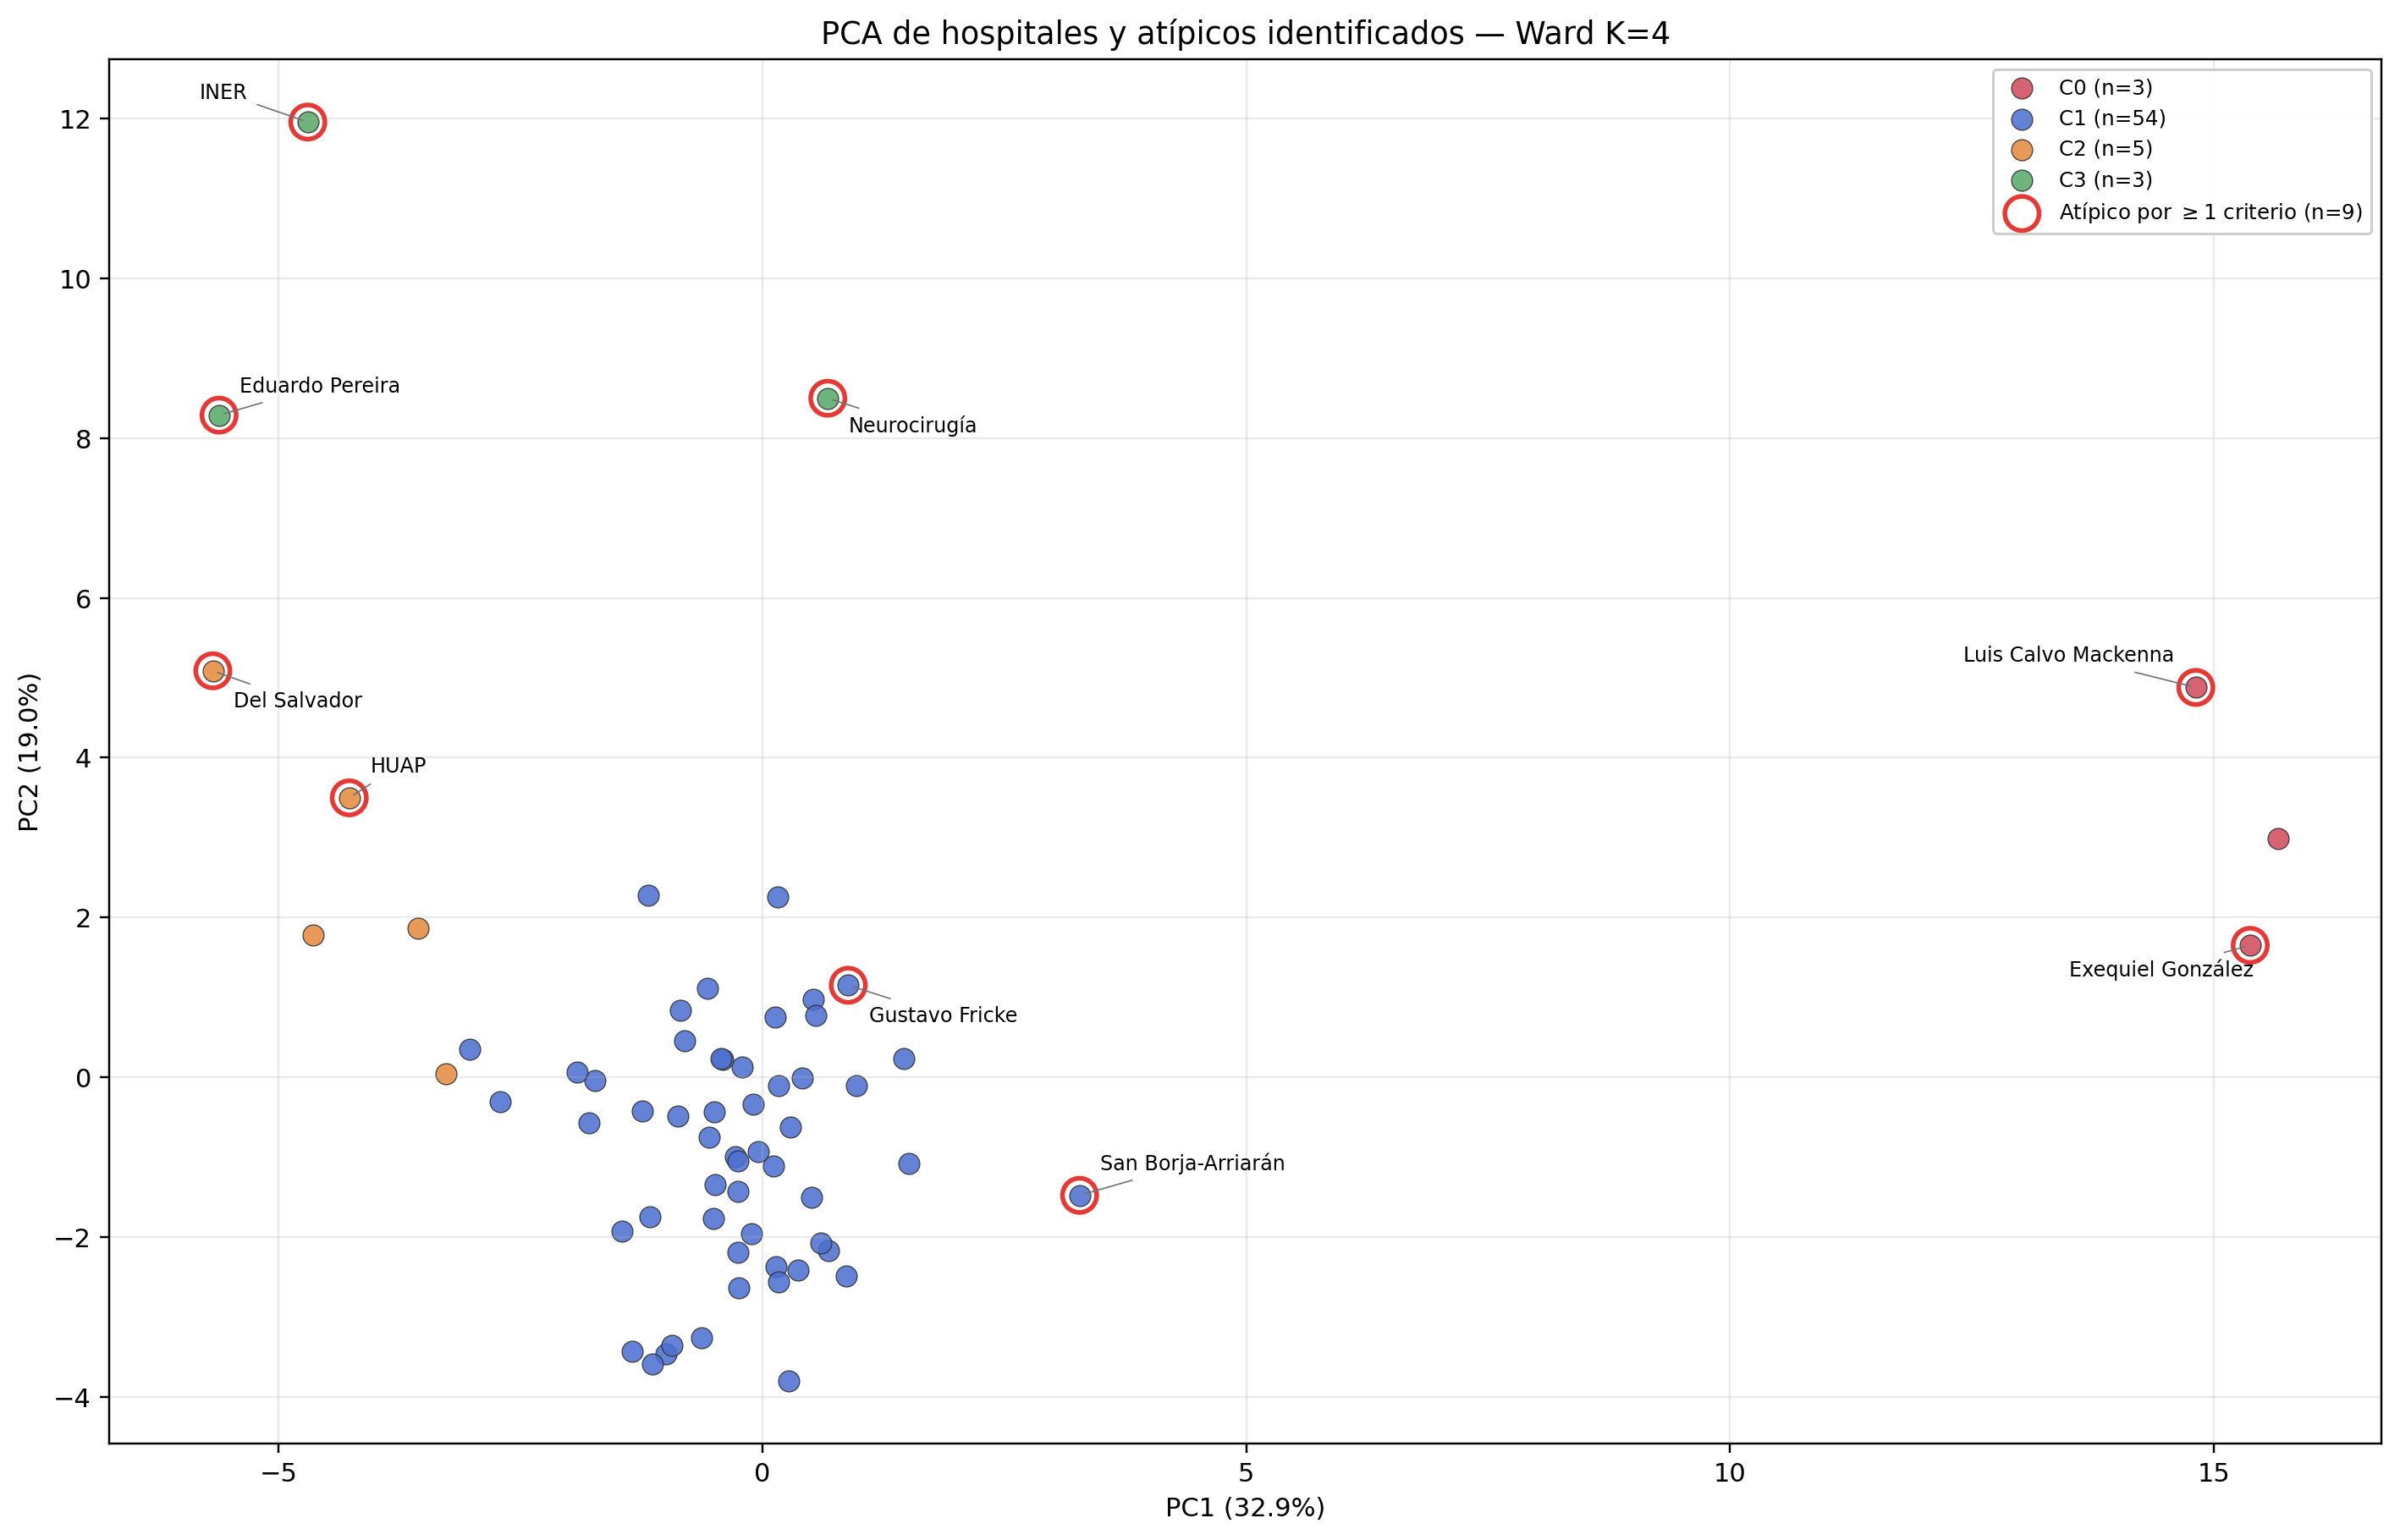
\includegraphics[width=\textwidth]{img/atipicos_pca.png}
\caption{Proyección PCA de los establecimientos, partición Ward $K=4$. Los círculos rojos indican hospitales atípicos.}
\label{fig:outliers-pca}
\end{figure}


\section{Sensibilidad algorítmica, temporal y composicional}

\label{sec:sensibilidad-analisis}

Antes de presentar los resultados, es necesario delimitar el alcance de estas comparaciones. Los algoritmos alternativos, las proyecciones bidimensionales y la solución Ward principal se construyen sobre la misma matriz de 35 variables y el mismo conjunto de 65 hospitales. Por ello, las comparaciones algorítmicas corresponden a un análisis de sensibilidad interna y no a una validación externa. Una validación externa requeriría contrastar la partición con hospitales, períodos o fuentes de información no utilizados en su construcción, lo que no se dispone en este estudio.

La proyección PCA presentada en la Sección~\ref{sec:res-outliers} tiene un propósito exploratorio y descriptivo. Permite observar una representación bidimensional de las mismas etiquetas Ward, pero no constituye un algoritmo alternativo de clustering ni evidencia independiente de la estabilidad de la partición. Por esta razón, la sensibilidad algorítmica se evalúa mediante MST-kNN, K-means y mezclas gaussianas, junto con índices cuantitativos de concordancia entre particiones.

\subsection*{Sensibilidad frente al algoritmo MST-kNN}

Se aplicó el algoritmo MST-kNN~\citep{inostroza2008} sobre la misma matriz institucional utilizada por Ward, explorando valores de $k$ entre 3 y 8 en modo mutuo. En esta configuración, dos hospitales se consideran vecinos solo cuando la relación de vecindad es recíproca. El algoritmo no impone un número fijo de grupos y puede producir grupos unitarios o pares, por lo que sus resultados no son directamente equivalentes a una partición de cuatro clústeres.

La Tabla~\ref{tab:mstknn-sensibilidad} presenta el comportamiento de la solución al variar $k$. A medida que aumenta el número de vecinos, disminuyen los grupos descubiertos y los grupos unitarios, mientras que el bloque de mayor tamaño aumenta desde 23 hospitales con $k=3$ hasta 38 con $k=8$. Esto muestra que la granularidad obtenida mediante MST-kNN depende de la definición de vecindad seleccionada.

\begin{table}[htbp]
\centering
\caption{Resultados del análisis de sensibilidad con MST-kNN en modo mutuo.}
\label{tab:mstknn-sensibilidad}

\begin{tabular}{c c c c c l}
\toprule
\textbf{$k$} & \textbf{$K$ total} & \textbf{Grupos $n\geq3$} & \textbf{Pares} & \textbf{Unitarios} & \textbf{Tamaños de grupos $n\geq3$} \\
\midrule
3 & 26 & 5 & 6 & 15 & [23, 5, 4, 3, 3] \\
4 & 25 & 5 & 6 & 14 & [23, 5, 5, 3, 3] \\
5 & 22 & 5 & 7 & 10 & [25, 5, 5, 3, 3] \\
6 & 21 & 5 & 6 & 10 & [27, 5, 5, 3, 3] \\
7 & 17 & 5 & 5 & 7 & [34, 5, 3, 3, 3] \\
8 & 14 & 5 & 4 & 5 & [38, 5, 3, 3, 3] \\
\bottomrule
\end{tabular}
\end{table}

Entre las configuraciones exploradas, $k=8$ alcanza el mayor Silhouette interno ($0{,}075$), aunque mantiene 14 grupos, incluidos cinco grupos unitarios. Por otro lado, $k=6$ genera 21 grupos, cinco de ellos con al menos tres hospitales, seis pares y diez grupos unitarios. Ninguna de estas configuraciones reproduce una partición compacta de cuatro grupos comparable directamente con Ward. En consecuencia, MST-kNN se interpreta como una sensibilidad a una definición local de vecindad y no como un método destinado a seleccionar una solución alternativa única.

El resultado principal del barrido es que el núcleo generalista no permanece como un bloque único al exigir vecindades mutuas locales. Dependiendo de $k$, este núcleo se divide en un grupo principal, grupos pequeños y hospitales unitarios. Esta diferencia es consistente con la naturaleza del método, que prioriza conexiones locales recíprocas y no minimiza la varianza intragrupo bajo el mismo criterio que Ward.

\subsection*{Concordancia cuantitativa entre particiones alternativas}

Para cuantificar la sensibilidad algorítmica, se calcularon el Índice de Rand Ajustado (ARI) y la Información Mutua Normalizada (NMI) entre la solución Ward $K=4$ y tres algoritmos alternativos construidos sobre la misma matriz: K-means con $K=4$, GMM con $K=4$ y MST-kNN con $k=6$ en modo mutuo. Además, se comparó el bloque generalista más grande mediante el índice de Jaccard y su recall respecto del núcleo generalista de Ward. Para los hospitales especializados, se calculó la proporción que permanece fuera del bloque principal de cada algoritmo alternativo. Los resultados se presentan en la Tabla~\ref{tab:concordancia-sensibilidad}.

\begin{table}[htbp]
\centering
\caption{Concordancia cuantitativa entre la partición Ward $K=4$ y particiones alternativas.}
\label{tab:concordancia-sensibilidad}
\resizebox{\textwidth}{!}{%
\begin{tabular}{l c c c c c}
\toprule
\textbf{Partición alternativa} &
\textbf{ARI} &
\textbf{NMI} &
\textbf{Jaccard núcleo} &
\textbf{Recall núcleo} &
\textbf{Recall especializados fuera del núcleo} \\
\midrule
K-means ($K=4$) &
0,927 &
0,851 &
0,982 &
0,982 &
1,000 \\

GMM ($K=4$) &
0,314 &
0,520 &
0,546 &
0,556 &
0,909 \\

MST-kNN ($k=6$, mutuo) &
0,180 &
0,429 &
0,500 &
0,500 &
1,000 \\
\bottomrule
\end{tabular}%
}
\end{table}

K-means presenta una concordancia alta con Ward, con $\text{ARI}=0{,}927$ y $\text{NMI}=0{,}851$. El bloque principal de K-means contiene 53 de los 54 hospitales del núcleo generalista Ward, y todos los hospitales especializados permanecen fuera de dicho bloque. Esta coincidencia es informativa, aunque debe interpretarse considerando que K-means y Ward comparten una preferencia por grupos compactos bajo distancia euclidiana. Por tanto, no constituyen mecanismos completamente independientes.

GMM y MST-kNN muestran una concordancia menor con la partición completa. Para GMM, el ARI es $0{,}314$ y el NMI es $0{,}520$; para MST-kNN, el ARI es $0{,}180$ y el NMI es $0{,}429$. Estos resultados indican que ambos algoritmos reorganizan una parte relevante de la partición Ward, especialmente dentro del núcleo generalista. En efecto, el recall del núcleo generalista es $0{,}556$ para GMM y $0{,}500$ para MST-kNN.

La separación entre el núcleo generalista y los hospitales especializados presenta una persistencia mayor que la composición interna del núcleo. MST-kNN mantiene a todos los hospitales especializados fuera de su bloque principal, mientras que GMM mantiene fuera a $90{,}9\%$ de ellos. Esta evidencia no implica que los grupos especializados se reproduzcan de manera idéntica entre métodos, sino que su diferenciación respecto del bloque generalista tiende a conservarse mejor que las fronteras internas del núcleo.

En conjunto, los resultados describen una sensibilidad algorítmica asimétrica. La distinción entre hospitales especializados y el núcleo generalista se mantiene en mayor medida bajo mecanismos alternativos, mientras que la asignación detallada de los hospitales que integran el núcleo generalista depende más del algoritmo utilizado.

\subsection*{Sensibilidad temporal: exclusión de los años de pandemia (2020--2021)}

Siguiendo el procedimiento descrito en la Sección~\ref{sec:sensibilidad-temporal}, se reconstruyó la matriz institucional excluyendo los años 2020 y 2021, manteniendo el mismo universo de 65 hospitales. Posteriormente, se aplicó nuevamente Ward con $K=4$ y se comparó la partición obtenida con la solución construida sobre el período completo 2019--2024.

La solución sin pandemia presenta un Silhouette de $0{,}356$ y tamaños de grupo $[3,51,2,9]$, frente al Silhouette de $0{,}400$ y los tamaños $[3,54,5,3]$ de la partición principal. La concordancia entre ambas soluciones alcanza $\text{ARI}=0{,}809$ y $\text{NMI}=0{,}750$, lo que indica una estabilidad importante, aunque no completa. La distribución de las reasignaciones se detalla en la Tabla~\ref{tab:contingencia-temporal}.

\begin{table}[htbp]
\centering
\caption{Contingencia entre la partición Ward $K=4$ (período completo) y la solución sin 2020--2021.}
\label{tab:contingencia-temporal}
\begin{tabular}{c c c c c}
\toprule
\textbf{Original $\backslash$ Sin pandemia} & \textbf{0} & \textbf{1} & \textbf{2} & \textbf{3} \\
\midrule
\textbf{0} ($C0$) & 3 & 0 & 0 & 0 \\
\textbf{1} ($C1$) & 0 & 51 & 0 & 3 \\
\textbf{2} ($C2$) & 0 & 0 & 0 & 5 \\
\textbf{3} ($C3$) & 0 & 0 & 2 & 1 \\
\bottomrule
\end{tabular}
\end{table}

Los tres hospitales de $C0$ permanecen agrupados al excluir los años de pandemia. En el núcleo generalista, 51 de los 54 hospitales permanecen en el bloque principal de la solución temporal alternativa, mientras que tres se reasignan a otro grupo. Los cambios restantes se concentran en los grupos pequeños $C2$ y $C3$. Por tanto, la estructura global se conserva en términos generales, pero los límites entre los perfiles de menor tamaño son más sensibles a la ventana temporal considerada.

La sensibilidad temporal por variable se concentra especialmente en algunas componentes de casuística. Las componentes \texttt{dim\_07} y \texttt{dim\_08} presentan cambios relativos medianos de $124{,}7\%$ y $104{,}7\%$, respectivamente, mientras que \texttt{tasa\_partos} presenta un cambio relativo mediano de $41{,}0\%$. Estos resultados indican que las interpretaciones clínicas finas asociadas a componentes específicas del PCA son más sensibles a la exclusión de 2020--2021 que los perfiles funcionales globales.

Como contraste adicional, se ponderaron las ocho componentes por la raíz de su
varianza explicada: \texttt{dim\_01} explica $22{,}8\%$ y \texttt{dim\_08}
$3{,}4\%$. La ponderación mejoró las métricas internas (Silhouette de $0{,}401$
a $0{,}446$; Davies--Bouldin de $0{,}990$ a $0{,}881$), pero reorganizó tres
hospitales entre los dos grupos pequeños ($ARI=0{,}992$; $NMI=0{,}944$). Por
ello se mantiene la ponderación uniforme de la solución canónica y el resultado
ponderado se interpreta como evidencia de sensibilidad: la estructura global
persiste, pero las fronteras finas entre perfiles especializados dependen del
peso asignado a la casuística.

Los 65 hospitales del universo final poseen cobertura completa para los seis años del período analizado. En consecuencia, no se compararon hospitales con cobertura temporal completa e incompleta dentro de esta muestra, ya que dicha heterogeneidad fue removida previamente por el criterio de elegibilidad descrito en la Sección~\ref{sec:elegibilidad}.

\subsection*{Sensibilidad composicional: transformación CLR de la casuística}

Siguiendo el procedimiento descrito en la Sección~\ref{sec:sensibilidad-composicional}, se reconstruyó la representación de casuística aplicando una transformación CLR a los vectores composicionales antes del PCA. Esta alternativa considera explícitamente que las proporciones de capítulos diagnósticos, procedimientos y GRD forman composiciones sujetas a la restricción de suma constante.

La partición obtenida mediante CLR+PCA reproduce exactamente la asignación Ward principal: $\text{ARI}=1{,}000$, $\text{NMI}=1{,}000$ y cero hospitales cambian de clúster. Los tamaños de los grupos se mantienen en $[3,54,5,3]$, como confirma la Tabla~\ref{tab:contingencia-clr}.

\begin{table}[htbp]
\centering
\caption{Contingencia entre la partición Ward con PCA convencional y con CLR+PCA.}
\label{tab:contingencia-clr}
\begin{tabular}{c c c c c}
\toprule
\textbf{PCA convencional $\backslash$ CLR+PCA} & \textbf{0} & \textbf{1} & \textbf{2} & \textbf{3} \\
\midrule
\textbf{0} ($C0$) & 3 & 0 & 0 & 0 \\
\textbf{1} ($C1$) & 0 & 54 & 0 & 0 \\
\textbf{2} ($C2$) & 0 & 0 & 5 & 0 \\
\textbf{3} ($C3$) & 0 & 0 & 0 & 3 \\
\bottomrule
\end{tabular}
\end{table}

La solución CLR+PCA presenta un Silhouette de $0{,}438$, frente a $0{,}400$ con la representación convencional. Además, las ocho componentes principales explican $76{,}9\%$ de la varianza en la representación CLR, frente a $72{,}3\%$ con PCA convencional. Estas diferencias muestran que la transformación CLR mejora la representación de la casuística bajo estos indicadores, pero no modifica la identidad de los cuatro perfiles obtenidos.

Por tanto, la posible clausura de las proporciones no altera la partición principal en este conjunto de datos. Este resultado respalda la estabilidad de los perfiles funcionales frente a una alternativa composicionalmente adecuada, aunque no convierte la solución en una validación externa.

\subsection*{Sensibilidad al criterio de elegibilidad de hospitales}

Como análisis adicional, se eliminó el requisito de cobertura temporal completa y se reconstruyó la matriz sobre 72 hospitales. Al restringir la comparación a los 65 hospitales compartidos con el análisis principal, la concordancia alcanza $\text{ARI}=0{,}936$ y $\text{NMI}=0{,}909$. La solución ampliada presenta tamaños $[3,53,12,4]$ y un Silhouette de $0{,}347$.

La disminución de cohesión respecto de la solución principal ($0{,}400$) y la concentración de seis de los siete hospitales con cobertura parcial en un mismo grupo sugieren que la inclusión de establecimientos con series temporales incompletas introduce perfiles institucionales menos comparables con el resto de la muestra. El criterio de elegibilidad se mantiene, por tanto, como una decisión para asegurar comparabilidad temporal, sin atribuirle la creación artificial de la estructura principal.

\subsection*{Síntesis de los análisis de sensibilidad}

Los resultados de sensibilidad muestran patrones diferenciados según el tipo de perturbación aplicada. La transformación CLR conserva exactamente la partición principal, mientras que la exclusión de 2020--2021 reduce la concordancia a $\text{ARI}=0{,}809$ y reorganiza principalmente los grupos de menor tamaño. La ampliación del universo a 72 hospitales mantiene una concordancia alta con la solución principal, aunque reduce la cohesión interna y concentra los establecimientos con cobertura incompleta.

Frente al cambio de algoritmo, la evidencia es asimétrica. K-means presenta una concordancia elevada con Ward, mientras que GMM y MST-kNN reorganizan de forma más importante la partición completa. Sin embargo, ambos métodos tienden a conservar, en distinta magnitud, la separación entre el bloque generalista y los establecimientos especializados. En consecuencia, los perfiles especializados muestran mayor persistencia frente a cambios metodológicos que la composición detallada del núcleo generalista.

Finalmente, la sensibilidad temporal afecta especialmente algunas componentes de casuística y la proporción de egresos neonatales. Por ello, la interpretación de los perfiles funcionales globales cuenta con mayor respaldo que una lectura exhaustiva de las componentes específicas del PCA o de diferencias clínicas finas entre los grupos.
